\documentclass[12pt]{article}
\usepackage[utf8]{inputenc}
\usepackage{amsmath} %Use for math
\usepackage{graphicx} %Use for images
\usepackage{color} %Use for color
\usepackage[section]{placeins}
\setlength\parindent{0pt} % Removes all indentation from paragraphs
\setlength{\parskip}{1.3ex plus 0.5ex minus 0.3ex} %Vertical space between two para
\newcommand{\tab}[1]{\hspace{.2\textwidth}\rlap{#1}}


\title{Control System -Lab}
\author{Gaurang Belekar, 20bec015}
\date{March 2022}

\begin{document}

\maketitle
\begin{center}
\text{Under the Guidance of Dr.Jagadish N}
\end{center}
\pagebreak

%===============================
%.  Experiment 1
%===============================
\begin{center}
    \LARGE {EXPERIMENT NO : 1}
             
\end{center}

\section*{\textcolor{black}{AIM: }}
\text{To calculate steady state error in position of Type 0}

\section*{\textcolor{black}{Block Diagram :}}
\begin{figure}[!hth]
        \centering
        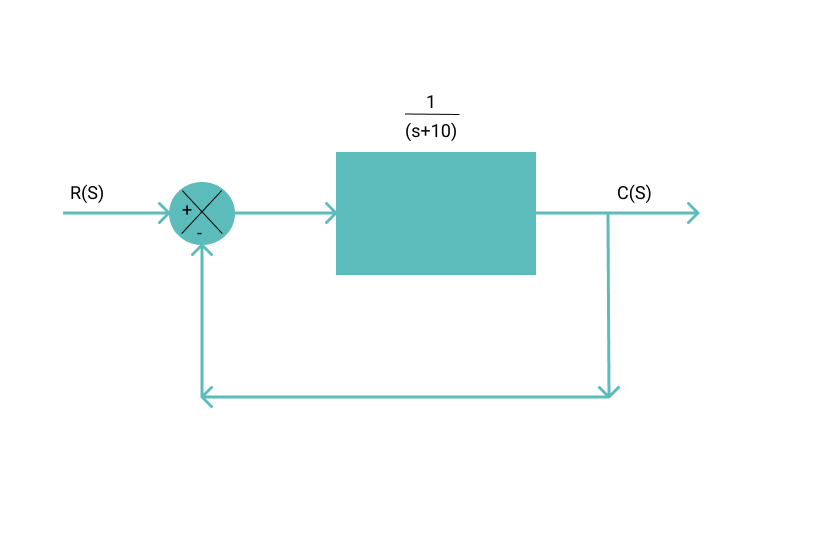
\includegraphics[width =10cm, height = 7cm]{images/exp1.png}
        \caption{Block Diagram}
        \label{Graph}
\end{figure}

\newline

\section*{\textcolor{black}{Theory :}}
Steady-state error is defined as the difference between the desired value and the actual value of a system output in the limit as time goes to infinity (i.e. when the response of the control system has reached steady-state).\par

Steady-state error is a property of the input/output response for a linear system. In general, a good control system will be one that has a low steady-state error
For a Type 0 system, the error is a non-zero, finite number, and Kp is equal to the Bode gain Kx. \par

\section*{\textcolor{black}{Code :}}

   s=\%s;\\ 
   g=syslin('c',1/(s+10))\\
   h=syslin('c',1/(0*s+1))\\
   G= g/.h\\
   t= 0:0.01:5;\\
   y= csim(t,t,G);\\
   plot(t,y)\\
   disp('STEADY STATE ERROR Ess:')\\
   disp(max(t)-max(y)) \par 

\section*{\textcolor{black}{OUTPUT/OBSERVATIONS}}

\begin{figure}[!hth]
        \centering
        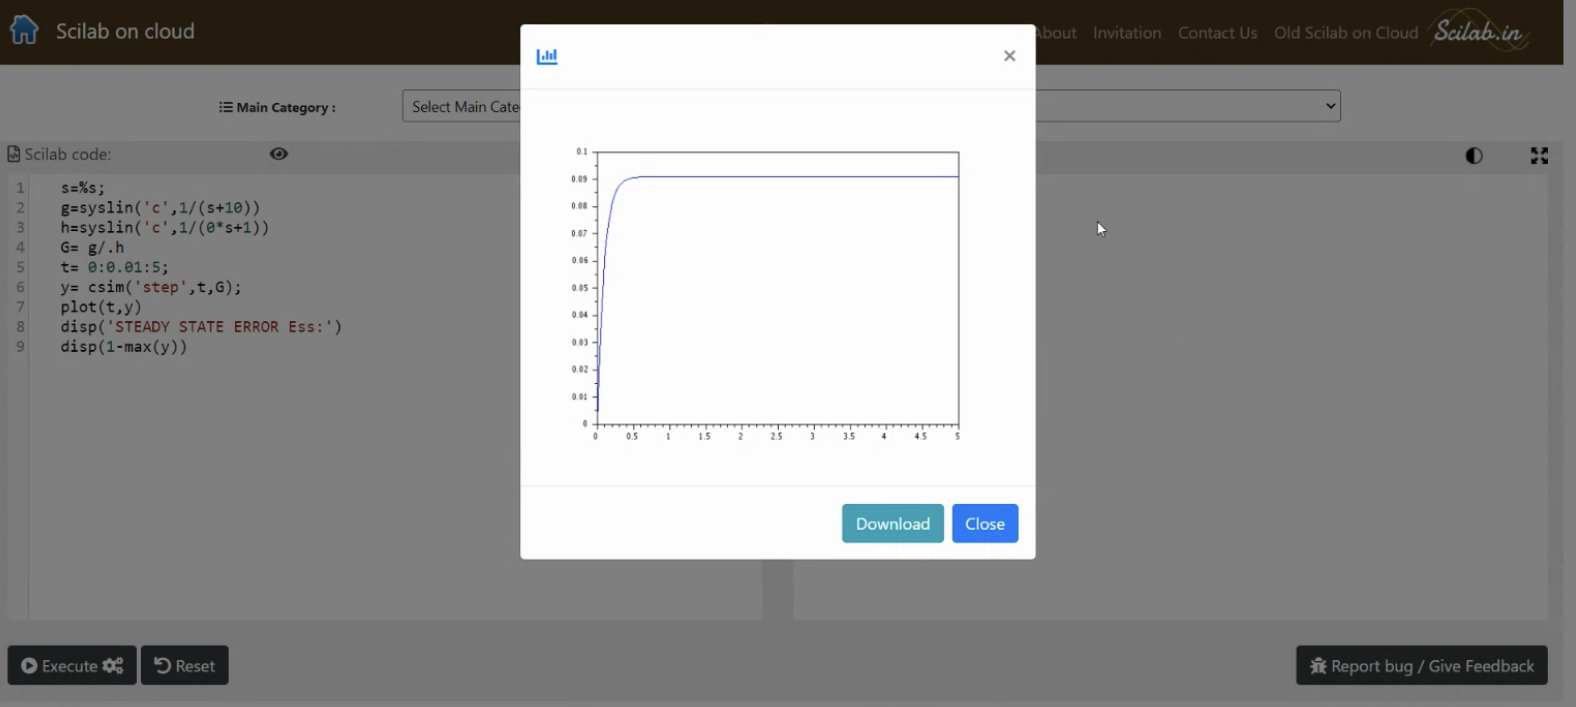
\includegraphics[width =10cm, height = 7cm]{images/exp11.png}
        \caption{Graph}
        \label{Graph}
\end{figure}
\begin{figure}[!hth]
        \centering
        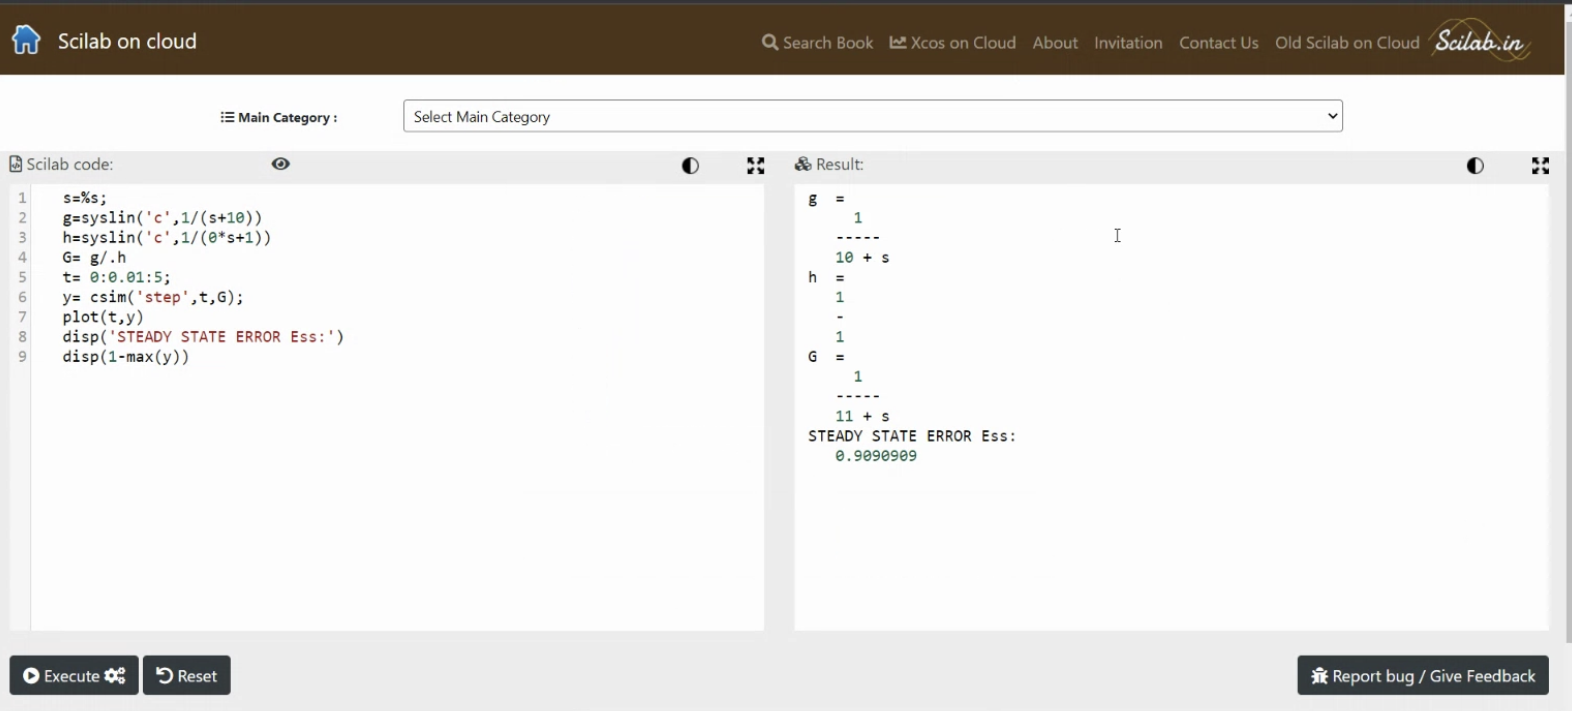
\includegraphics[width =10cm, height = 7cm]{images/exp12.png}
        \caption{Result}
        \label{Result}
\end{figure}

\section*{\textcolor{black}{Conclusion}}
We get a constant error of 0.909 in our case when we give step input in type 0.
 \pagebreak
 
%===============================
%.  Experiment 2
%===============================
\begin{center}
    \LARGE {EXPERIMENT NO : 2}
             
\end{center}

\section*{\textcolor{black}{AIM: }}
\text{To calculate steady state error in position of Type 0}

\section*{\textcolor{black}{Block Diagram :}}
\begin{figure}[!hth]
        \centering
        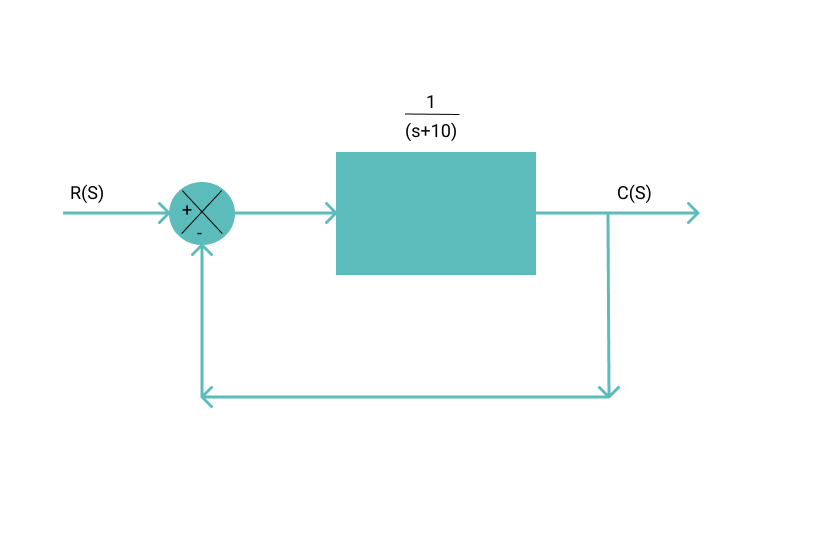
\includegraphics[width =10cm, height = 7cm]{images/exp2.png}
        \caption{Block Diagram}
        \label{Graph}
\end{figure}

\section*{\textcolor{black}{Theory :}}
Steady-state error is defined as the difference between the desired value and the actual value of a system output in the limit as time goes to infinity (i.e. when the response of the control system has reached steady-state).\par

Steady-state error is a property of the input/output response for a linear system. In general, a good control system will be one that has a low steady-state error
For a Type 0 system, the error is a non-zero, finite number, and Kp is equal to the Bode gain Kx. \par

\section*{\textcolor{black}{Code :}}

   s=\%s;\\ 
   g=syslin('c',1/(s+10))\\
   h=syslin('c',1/(0*s+1))\\
   G= g/.h\\
   t= 0:0.01:5;\\
   y= csim('step',t,G);\\
   plot(t,y)\\
   disp('STEADY STATE ERROR Ess:')\\
   disp(1-max(y)) \par 

\section*{\textcolor{black}{OUTPUT/OBSERVATIONS}}

\begin{figure}[!hth]
        \centering
        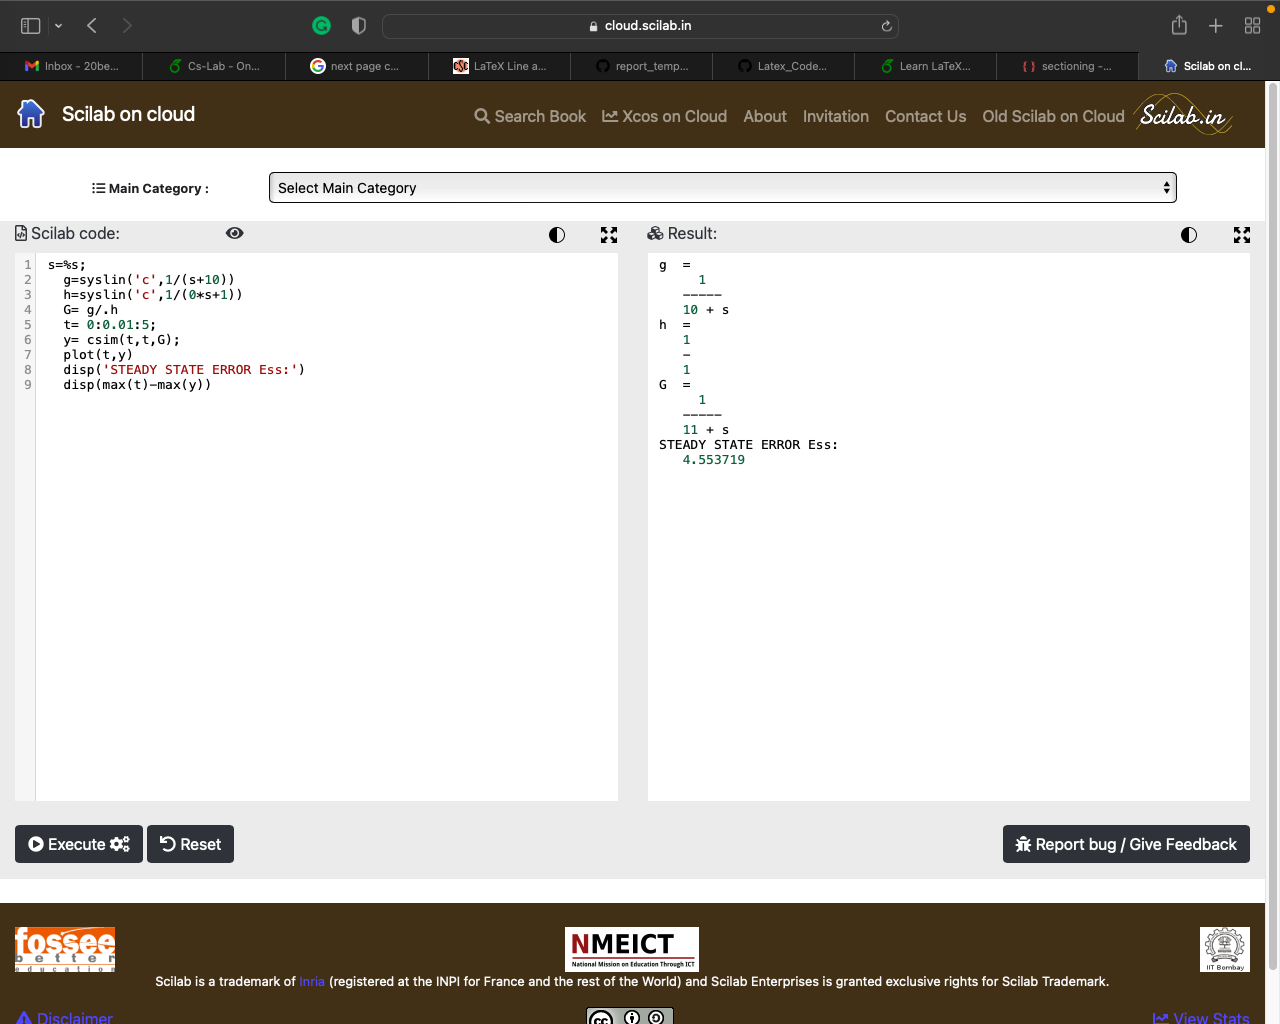
\includegraphics[width =10cm, height = 7cm]{images/exp21.png}
        \caption{Graph}
        \label{Graph}
\end{figure}
\begin{figure}[!hth]
        \centering
        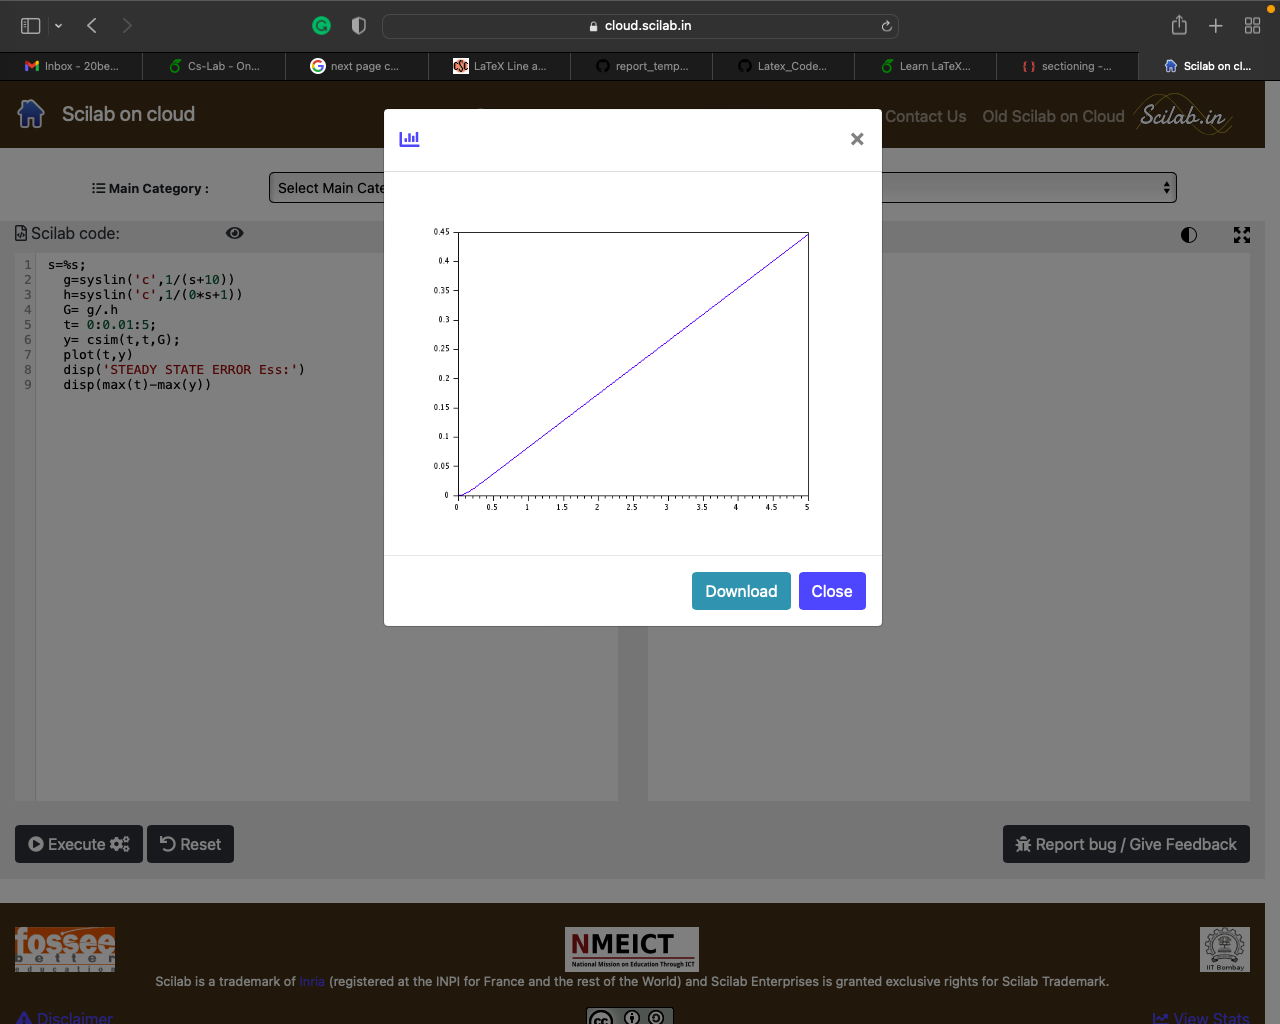
\includegraphics[width =10cm, height = 7cm]{images/exp22.png}
        \caption{Result}
        \label{Result}
\end{figure}

\section*{\textcolor{black}{Conclusion}}
We get a straigth line passing from origin when we give ramp input in type
0 and as we keep on increasing time we get infinte value difference.
\pagebreak
 
 
 
 %===============================
%.  Experiment 3
%===============================
\begin{center}
    \LARGE {EXPERIMENT NO : 3}
             
\end{center}

\section*{\textcolor{black}{AIM: }}
\text{To calculate steady state error in position of Type 0}

\section*{\textcolor{black}{Block Diagram :}}
\begin{figure}[!hth]
        \centering
        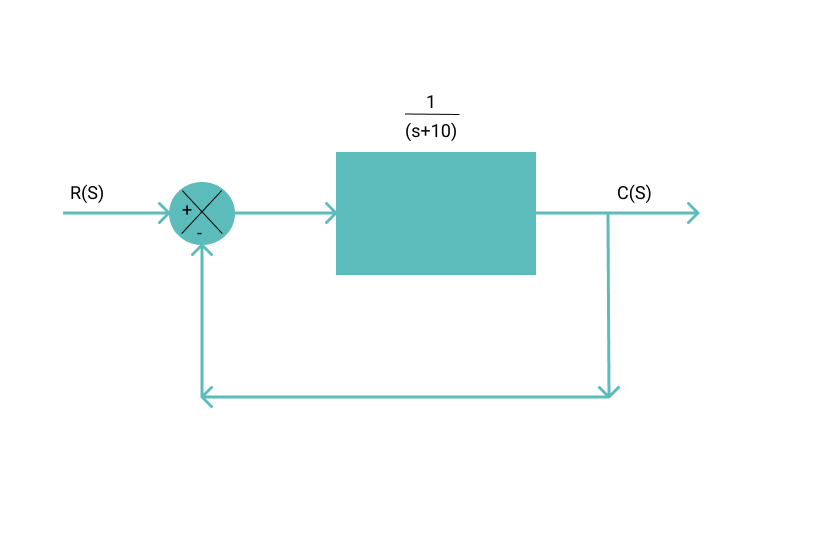
\includegraphics[width =10cm, height = 7cm]{images/exp3.png}
        \caption{Block Diagram}
        \label{Graph}
\end{figure}
\section*{\textcolor{black}{Theory :}}
Steady-state error is defined as the difference between the desired value and the actual value of a system output in the limit as time goes to infinity (i.e. when the response of the control system has reached steady-state).\par

Steady-state error is a property of the input/output response for a linear system. In general, a good control system will be one that has a low steady-state error
For a Type 0 system, the error is a non-zero, finite number, and Kp is equal to the Bode gain Kx. \par

\section*{\textcolor{black}{Code :}}

    s=\%s;\\ 
   g=syslin('c',1/(s+10))\\
   h=syslin('c',1/(0*s+1))\\
   G= g/.h\\
   t= 0:0.01:5;\\
   y= csim(t.\wedge2,t,G);\\
   plot(t,y)\\
   disp('STEADY STATE ERROR Ess:')\\
   disp(max(t.\wedge2)-max(y)) \par 

\section*{\textcolor{black}{OUTPUT/OBSERVATIONS}}

\begin{figure}[!hth]
        \centering
        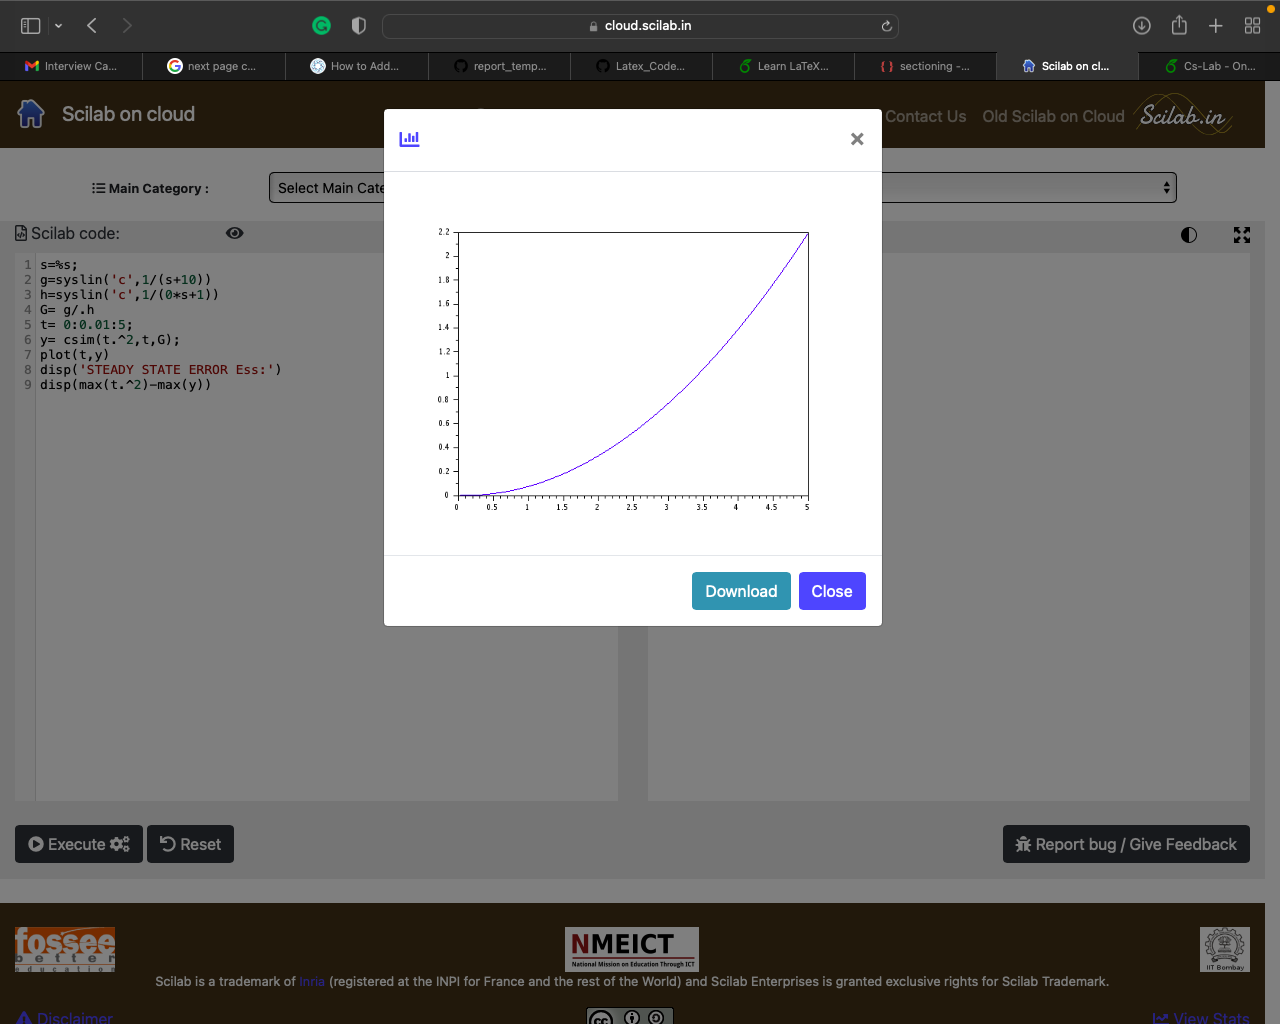
\includegraphics[width =10cm, height = 7cm]{images/exp31.png}
        \caption{Graph}
        \label{Graph}
\end{figure}
\begin{figure}[!hth]
        \centering
        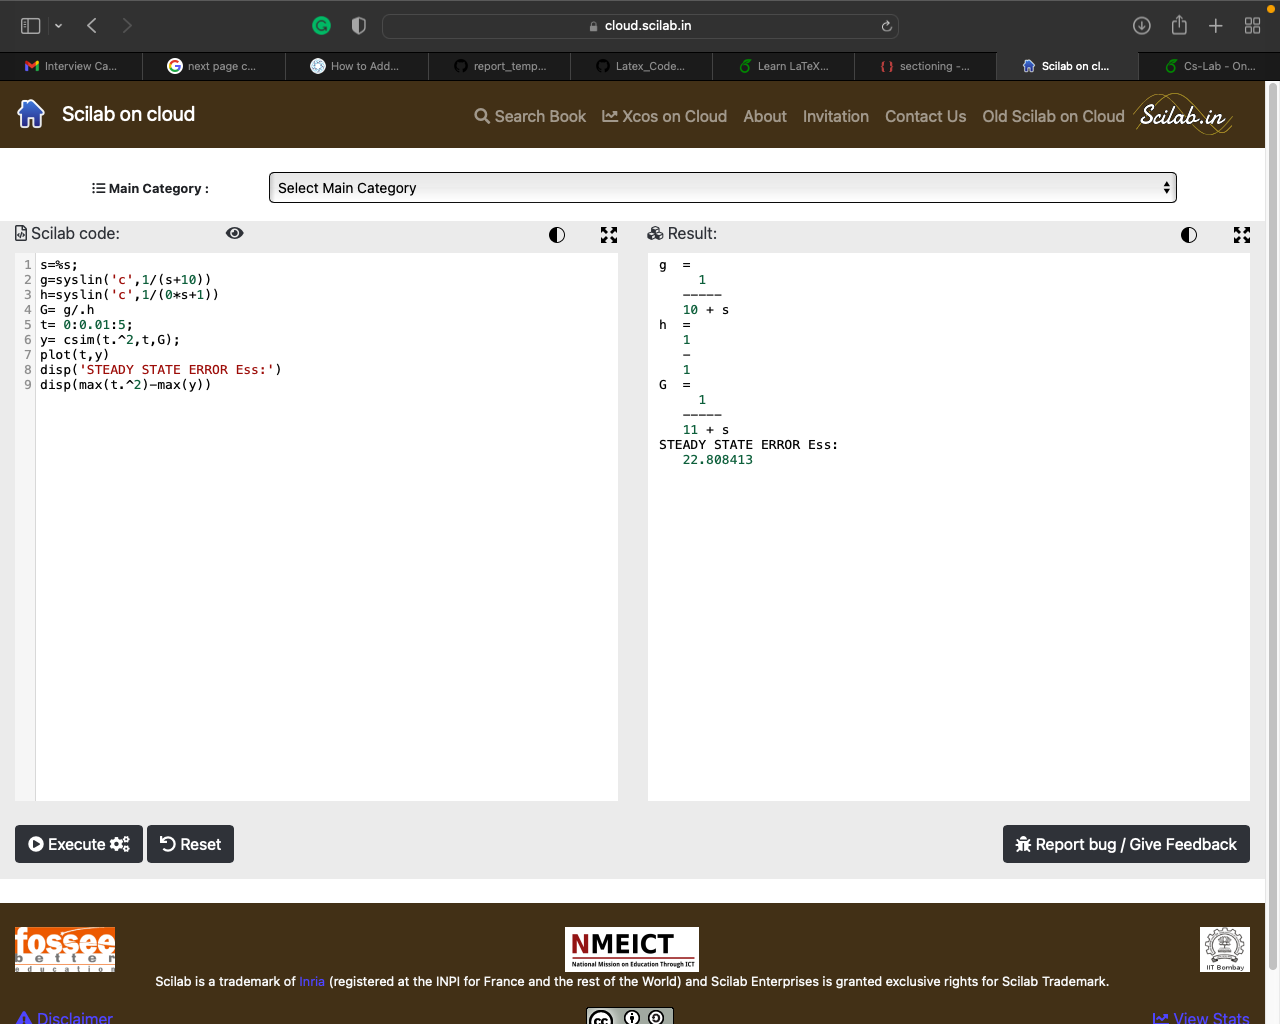
\includegraphics[width =10cm, height = 7cm]{images/exp32.png}
        \caption{Result}
        \label{Result}
\end{figure}

\section*{\textcolor{black}{Conclusion}}
 We get a parabolic curve when we give parabolic input in type 0 and as we keep on increasing time we get infinte value difference
 \pagebreak
 
 \begin{center}
    \LARGE {EXPERIMENT NO : 4}
             
\end{center}

\section*{\textcolor{black}{AIM: }}
\text{To calculate steady state error in position of Type 1}

\section*{\textcolor{black}{Block Diagram :}}
 \begin{figure}[!hth]
        \centering
        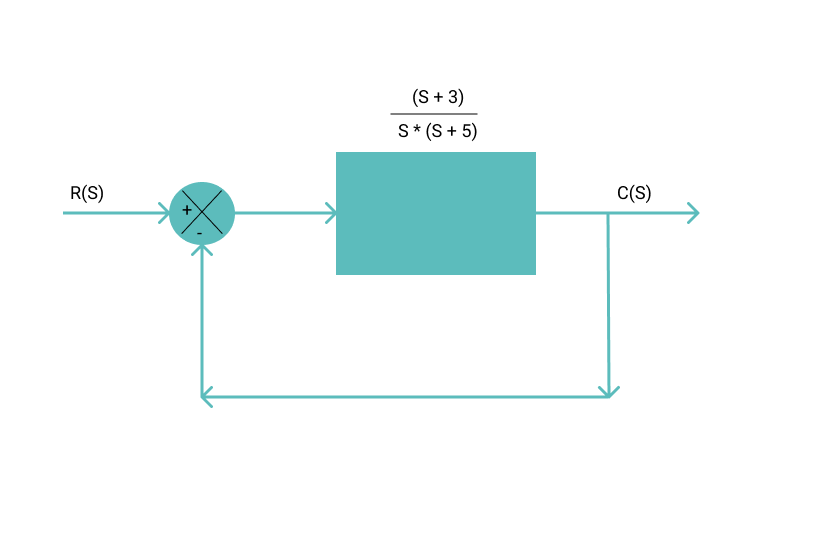
\includegraphics[width =10cm, height = 7cm]{images/exp4.png}
        \caption{Block Diagram}
        \label{Graph}
\end{figure}

\section*{\textcolor{black}{Theory :}}
Steady-state error is defined as the difference between the desired value and the actual value of a system output in the limit as time goes to infinity (i.e. when the response of the control system has reached steady-state).\par

Steady-state error is a property of the input/output response for a linear system. In general, a good control system will be one that has a low steady-state error
For a Type 0 system, the error is a non-zero, finite number, and Kp is equal to the Bode gain Kx. \par

\section*{\textcolor{black}{Code :}}

   s=\%s;\\ 
   g=syslin('c',(s+3)/s*(s+5))\\
   h=syslin('c',1/(0*s+1))\\
   G= g/.h\\
   t= 0:0.01:5;\\
   y= csim('step',t,G);\\
   plot(t,y)\\
   disp('STEADY STATE ERROR Ess:')\\
   disp(1-max(y)) \par 

\section*{\textcolor{black}{OUTPUT/OBSERVATIONS}}


\begin{figure}[!hth]
        \centering
        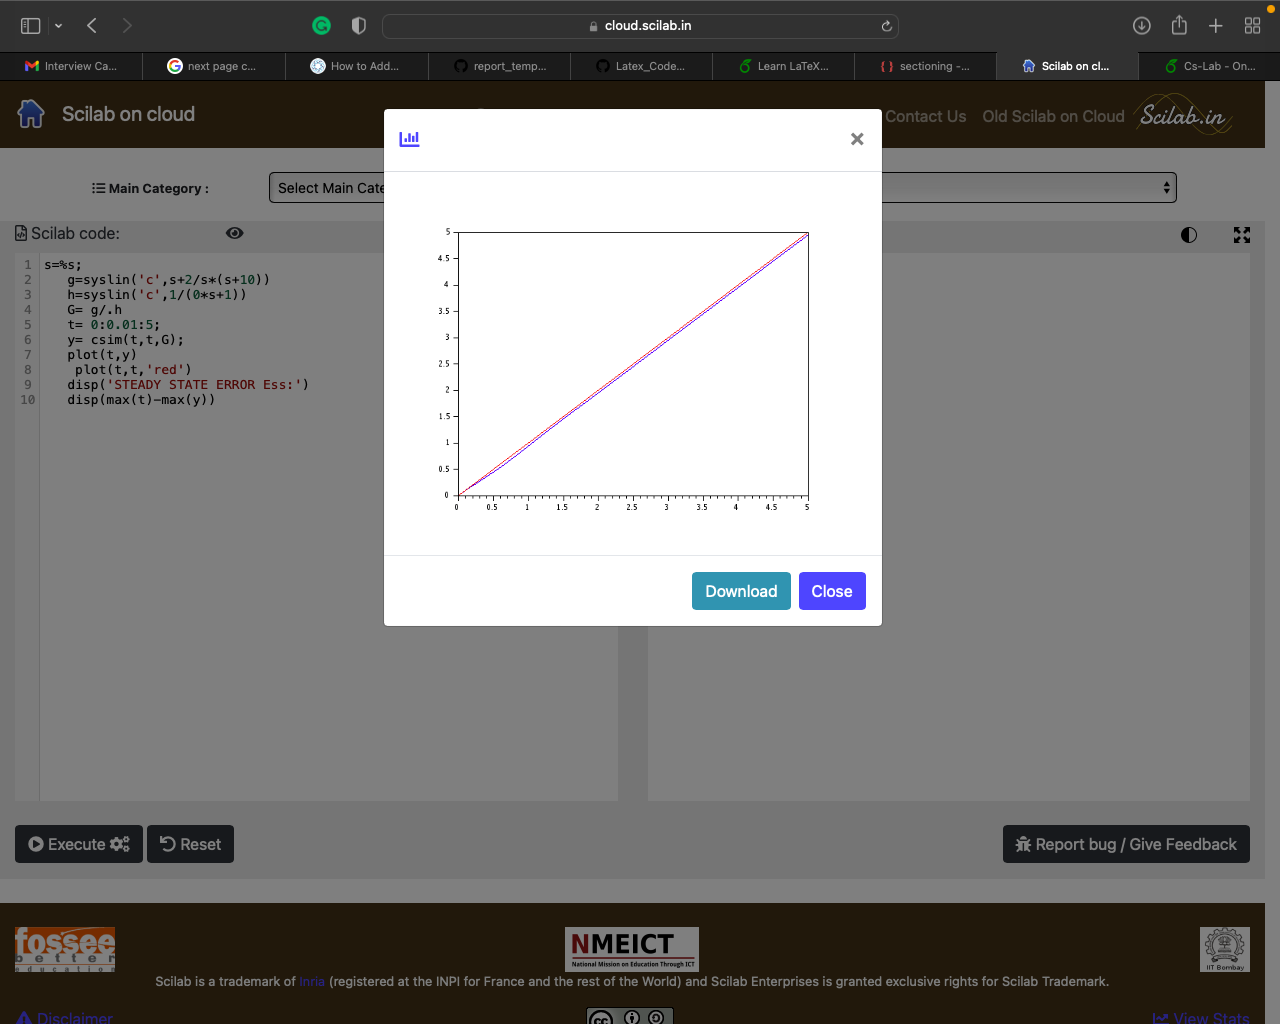
\includegraphics[width =10cm, height = 10cm]{images/exp41.png}
        \caption{Graph}
        \label{Result}
        
\end{figure}
        \begin{figure}[!hth]
        \centering
        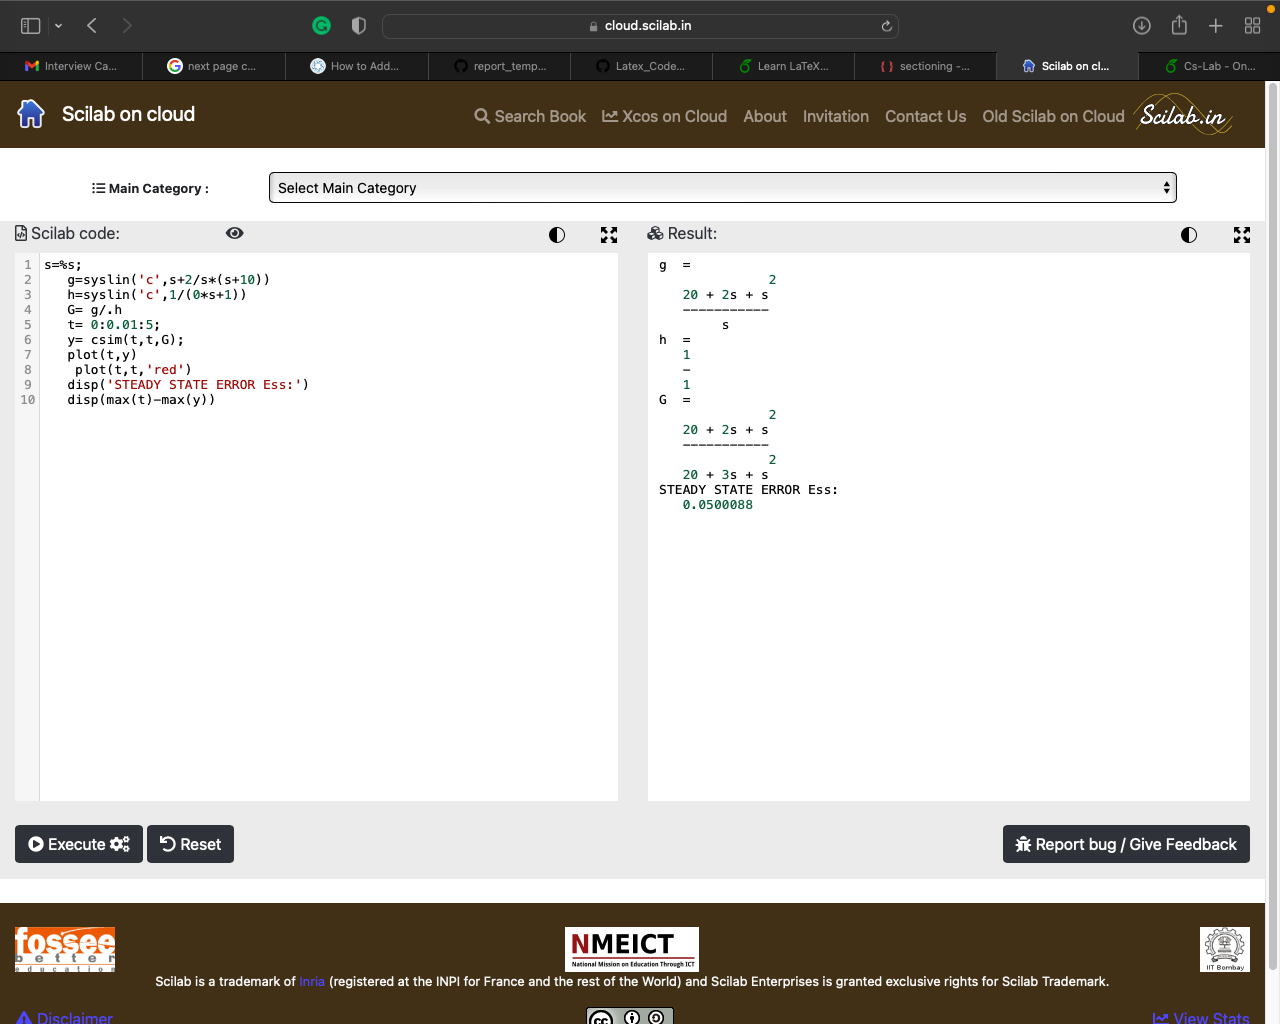
\includegraphics[width =10cm, height = 10cm]{images/exp42.png}
        \caption{Result}
        \label{Result}
\end{figure}

\section*{\textcolor{black}{Conclusion}}
We get a constant graph and as we increase the time , the error becomes 0 in case of step input in type 1.
  \pagebreak

\begin{center}
    \LARGE {EXPERIMENT NO : 5}
             
\end{center}

\section*{\textcolor{black}{AIM: }}
\text{To calculate steady state error in position of Type 1}

\section*{\textcolor{black}{Block Diagram :}}
\begin{figure}[!hth]
        \centering
        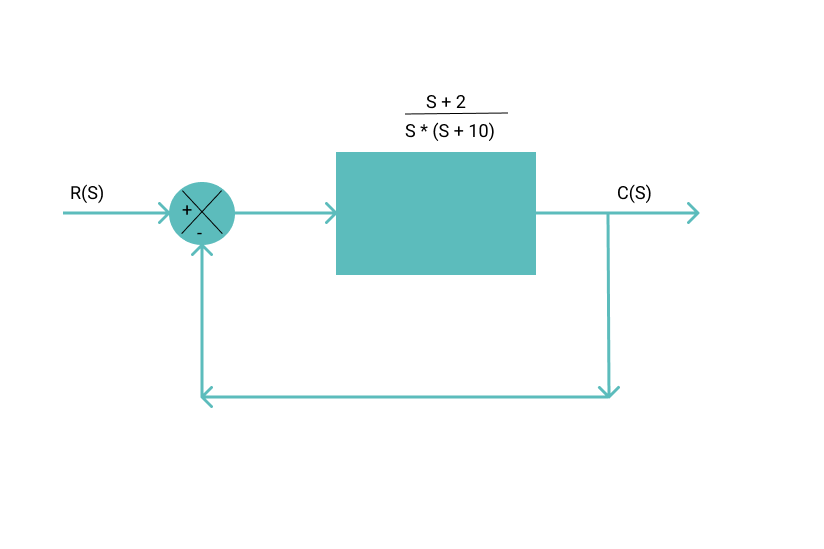
\includegraphics[width =10cm, height = 7cm]{images/exp5.png}
        \caption{Block Diagram}
        \label{Graph}
\end{figure}
\section*{\textcolor{black}{Theory :}}
Steady-state error is defined as the difference between the desired value and the actual value of a system output in the limit as time goes to infinity (i.e. when the response of the control system has reached steady-state).\par

Steady-state error is a property of the input/output response for a linear system. In general, a good control system will be one that has a low steady-state error
For a Type 0 system, the error is a non-zero, finite number, and Kp is equal to the Bode gain Kx. \par

\section*{\textcolor{black}{Code :}}

   s=\%s;\\ 
   g=syslin('c',s+2/s*(s+10))\\
   h=syslin('c',1/(0*s+1))\\
   G= g/.h\\
   t= 0:0.01:5;\\
   y= csim(t,t,G);\\
   plot(t,y)\\
    plot(t,t,'red')\\
   disp('STEADY STATE ERROR Ess:')\\
   disp(max(t)-max(y)) \par 

\section*{\textcolor{black}{OUTPUT/OBSERVATIONS}}

\begin{figure}[!hth]
        \centering
        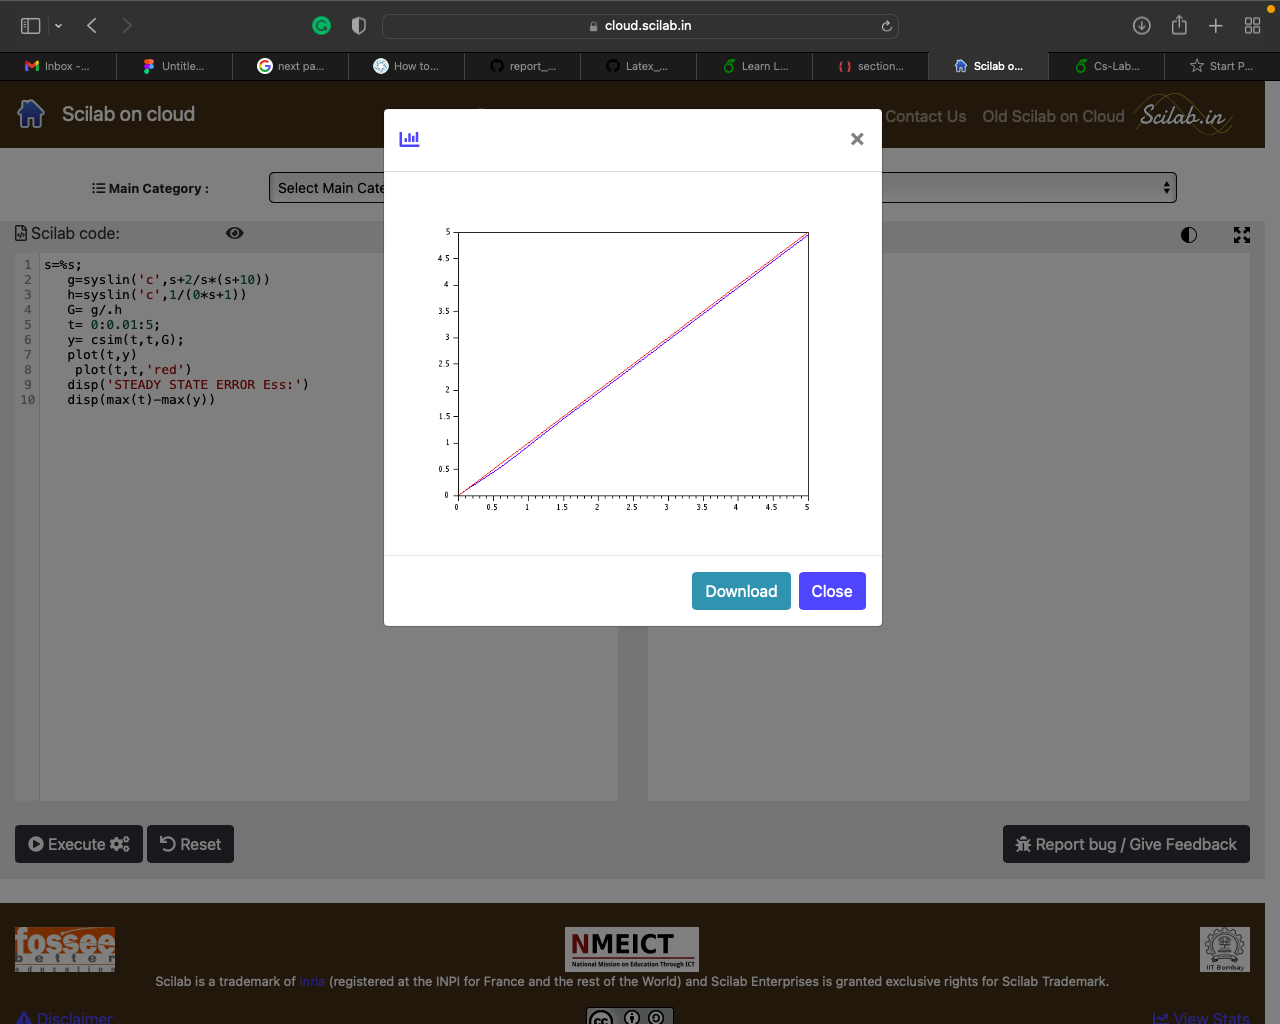
\includegraphics[width =10cm, height = 10cm]{images/exp51.png}
        \caption{Graph}
        \label{Graph}
\end{figure}
\begin{figure}[!hth]
        \centering
        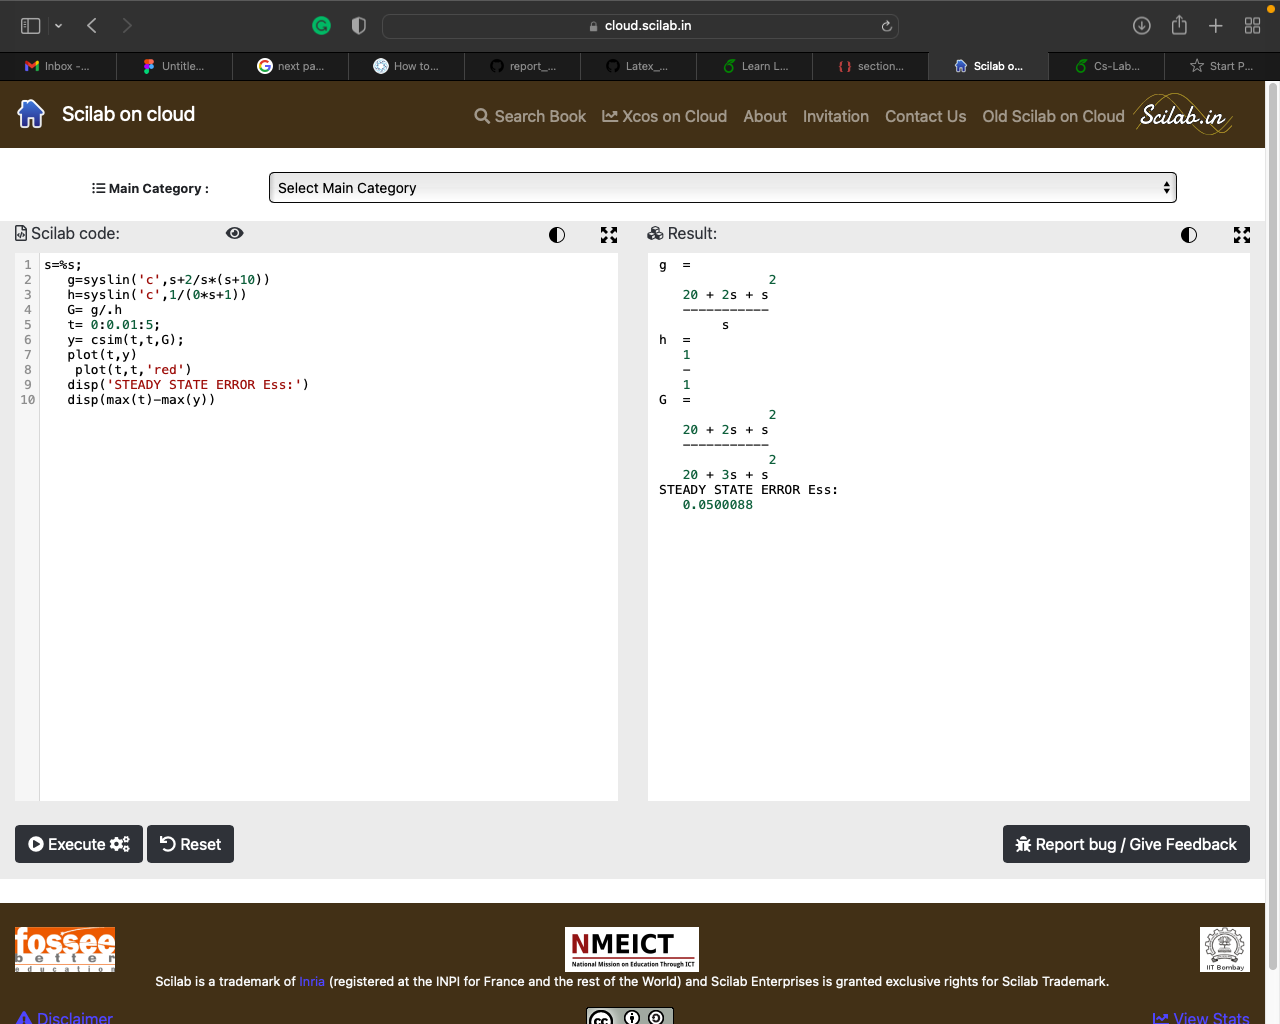
\includegraphics[width =10cm, height = 10cm]{images/exp52.png}
        \caption{Result}
        \label{Result}
\end{figure}

\section*{\textcolor{black}{Conclusion}}
We get a constant difference i.e. constant error which is equal to 1/Kv when we use ramp input in type 1.
 \pagebreak
 
 \begin{center}
    \LARGE {EXPERIMENT NO : 6}
             
\end{center}

\section*{\textcolor{black}{AIM: }}
\text{To calculate steady state error in acceleration of Type 1}

\section*{\textcolor{black}{Block Diagram :}}

\begin{figure}[!hth]
        \centering
        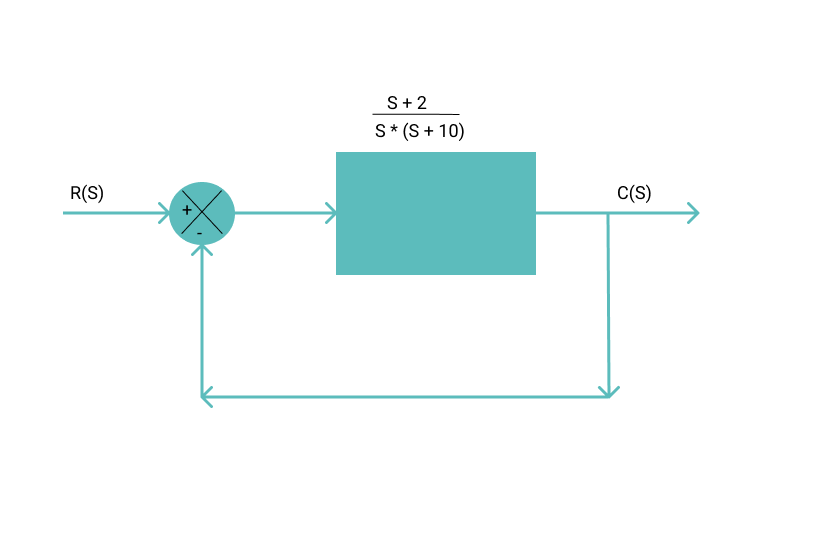
\includegraphics[width =10cm, height = 7cm]{images/exp6.png}
        \caption{Block Diagram}
        \label{Graph}
\end{figure}

\section*{\textcolor{black}{Theory :}}
Steady-state error is defined as the difference between the desired value and the actual value of a system output in the limit as time goes to infinity (i.e. when the response of the control system has reached steady-state).\par

Steady-state error is a property of the input/output response for a linear system. In general, a good control system will be one that has a low steady-state error
For a Type 0 system, the error is a non-zero, finite number, and Kp is equal to the Bode gain Kx. \par

\section*{\textcolor{black}{Code :}}

   s=\%s;\\ 
   g=syslin('c',(s+2)/s*(s+10))\\
   h=syslin('c',1/(0*s+1))\\
   G= g/.h\\
   t= 0:0.01:5;\\
   y= csim(t.\wedge2,t,G);\\
   plot(t,y)\\
    plot(t,t.\wedge2,'red')\\
   disp('STEADY STATE ERROR Ess:')\\
   disp(max(t.\wedge2)-max(y)) \par 

\section*{\textcolor{black}{OUTPUT/OBSERVATIONS}}

\begin{figure}[!hth]
        \centering
        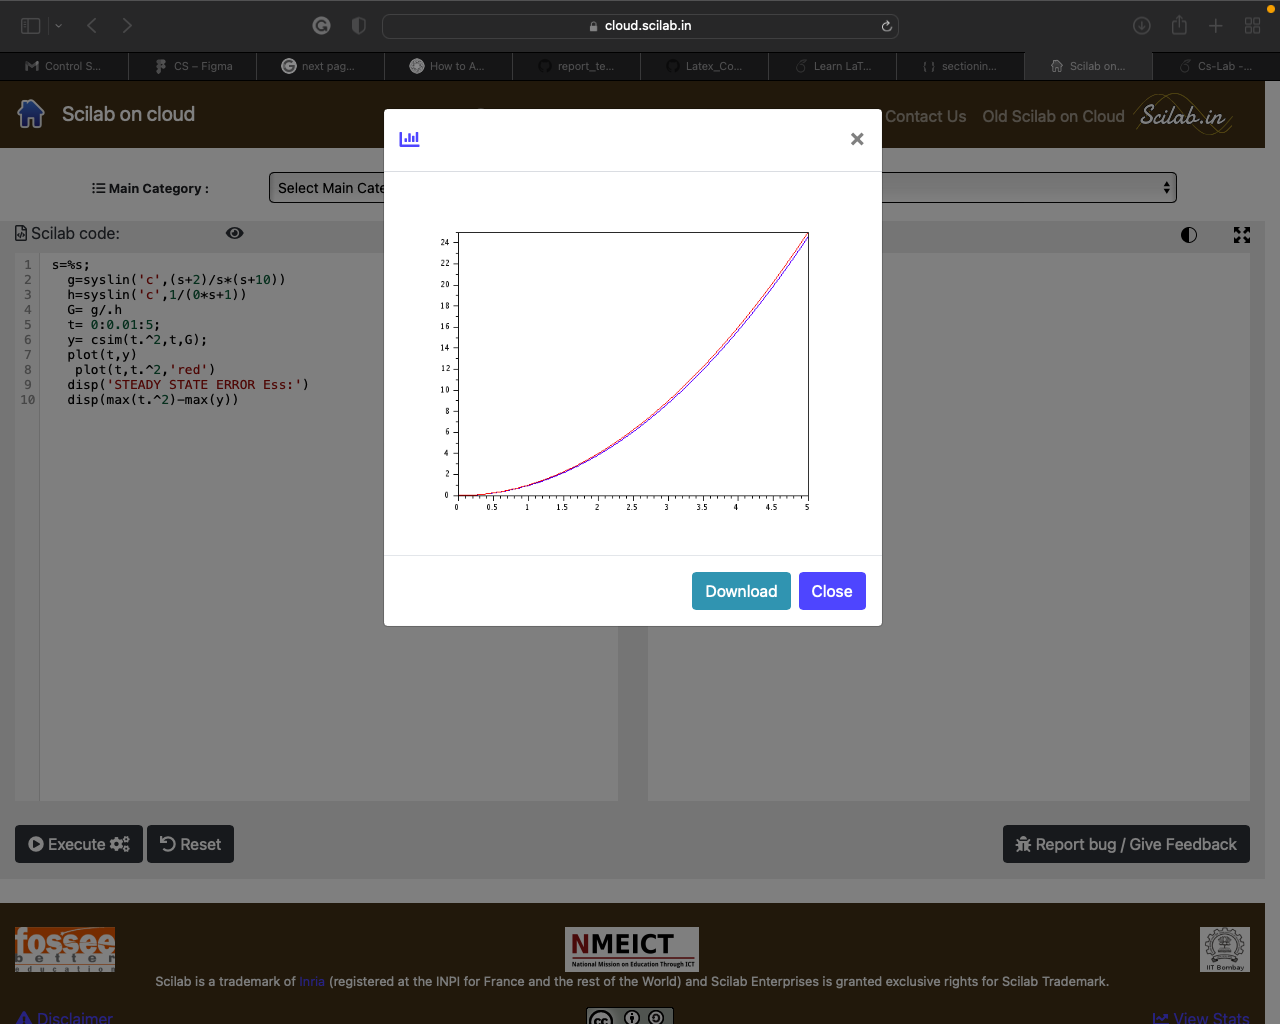
\includegraphics[width =10cm, height = 10cm]{images/exp61.png}
        \caption{Graph}
        \label{Graph}
\end{figure}
\begin{figure}[!hth]
        \centering
        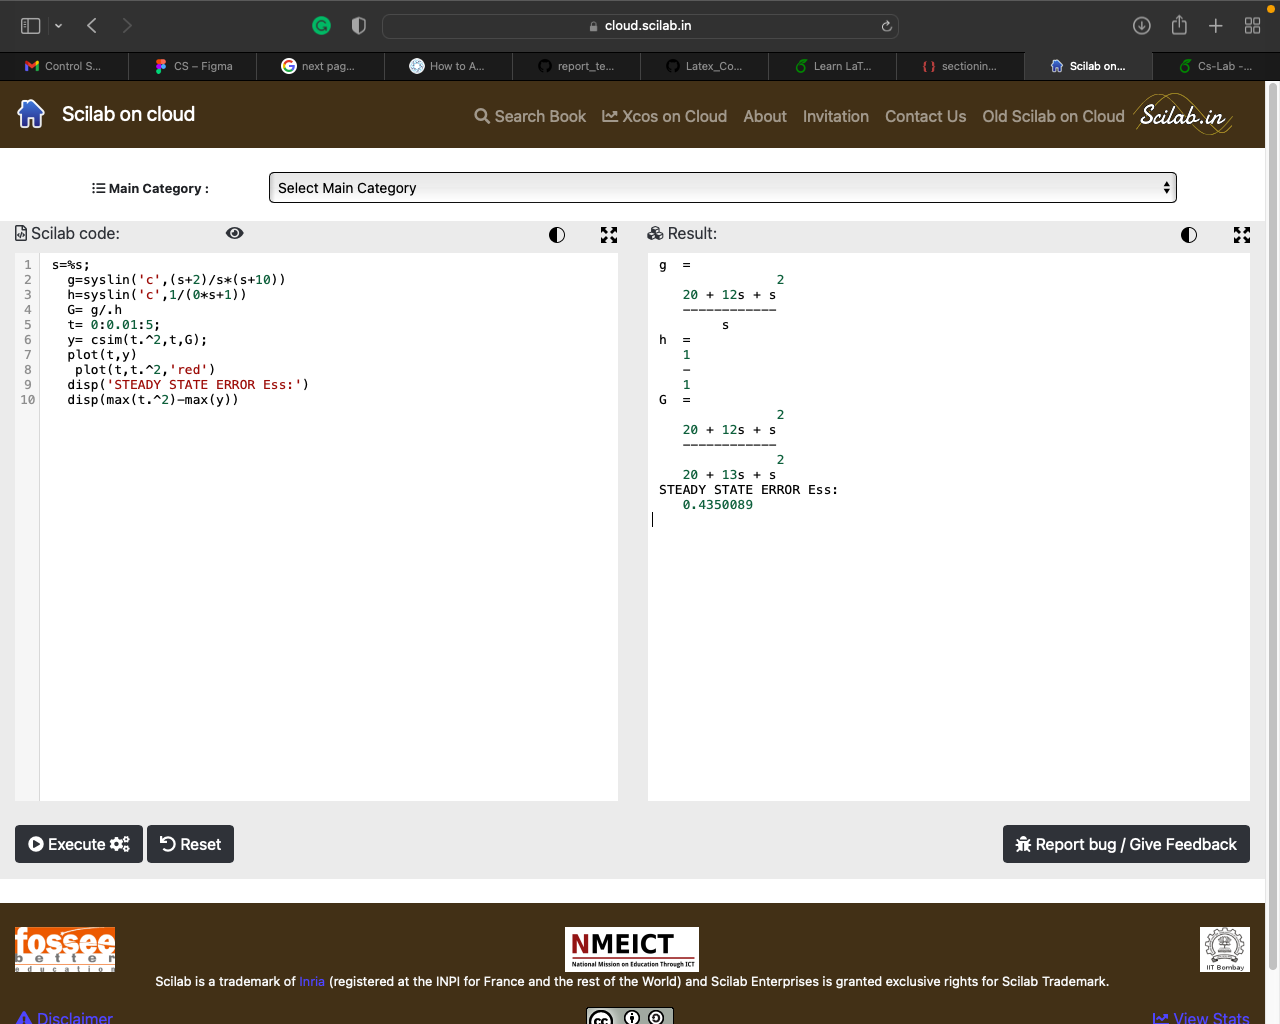
\includegraphics[width =10cm, height = 10cm]{images/exp62.png}
        \caption{Result}
        \label{Result}
\end{figure}


\section*{\textcolor{black}{Conclusion}}
 When we use a parabolic input in type 1 we get an increasing error which becomes infinite as we increase the time to infinite.
   \pagebreak
\maketitle
\begin{center}
    \LARGE {EXPERIMENT NO : 7}
             
\end{center}

\section*{\textcolor{black}{AIM: }}
\text{To calculate steady state error in position of Type 2}

\section*{\textcolor{black}{Block Diagram :}}

\begin{figure}[!hth]
        \centering
        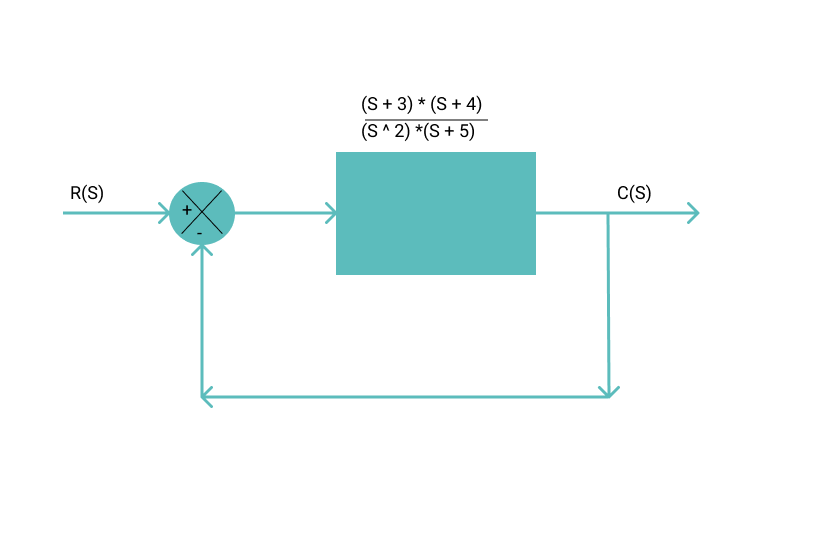
\includegraphics[width =10cm, height = 7cm]{images/exp7.png}
        \caption{Block Diagram}
        \label{Graph}
\end{figure}

\section*{\textcolor{black}{Theory :}}
Steady-state error is defined as the difference between the desired value and the actual value of a system output in the limit as time goes to infinity (i.e. when the response of the control system has reached steady-state).\par

Steady-state error is a property of the input/output response for a linear system. In general, a good control system will be one that has a low steady-state error
For a Type 0 system, the error is a non-zero, finite number, and Kp is equal to the Bode gain Kx. \par

\section*{\textcolor{black}{Code :}}

   s=\%s;\\ 
   g=syslin('c',(s+4)(s+3)/s.\wedge2(s+5))\\
   t= 0:0.01:5;\\
   y= csim('step',t,G);\\
   plot(t,y)\\
    plot(t,t,'red')\\
   disp('STEADY STATE ERROR Ess:')\\
   disp(1-max(y)) \par 

\section*{\textcolor{black}{OUTPUT/OBSERVATIONS}}

\begin{figure}[!hth]
        \centering
        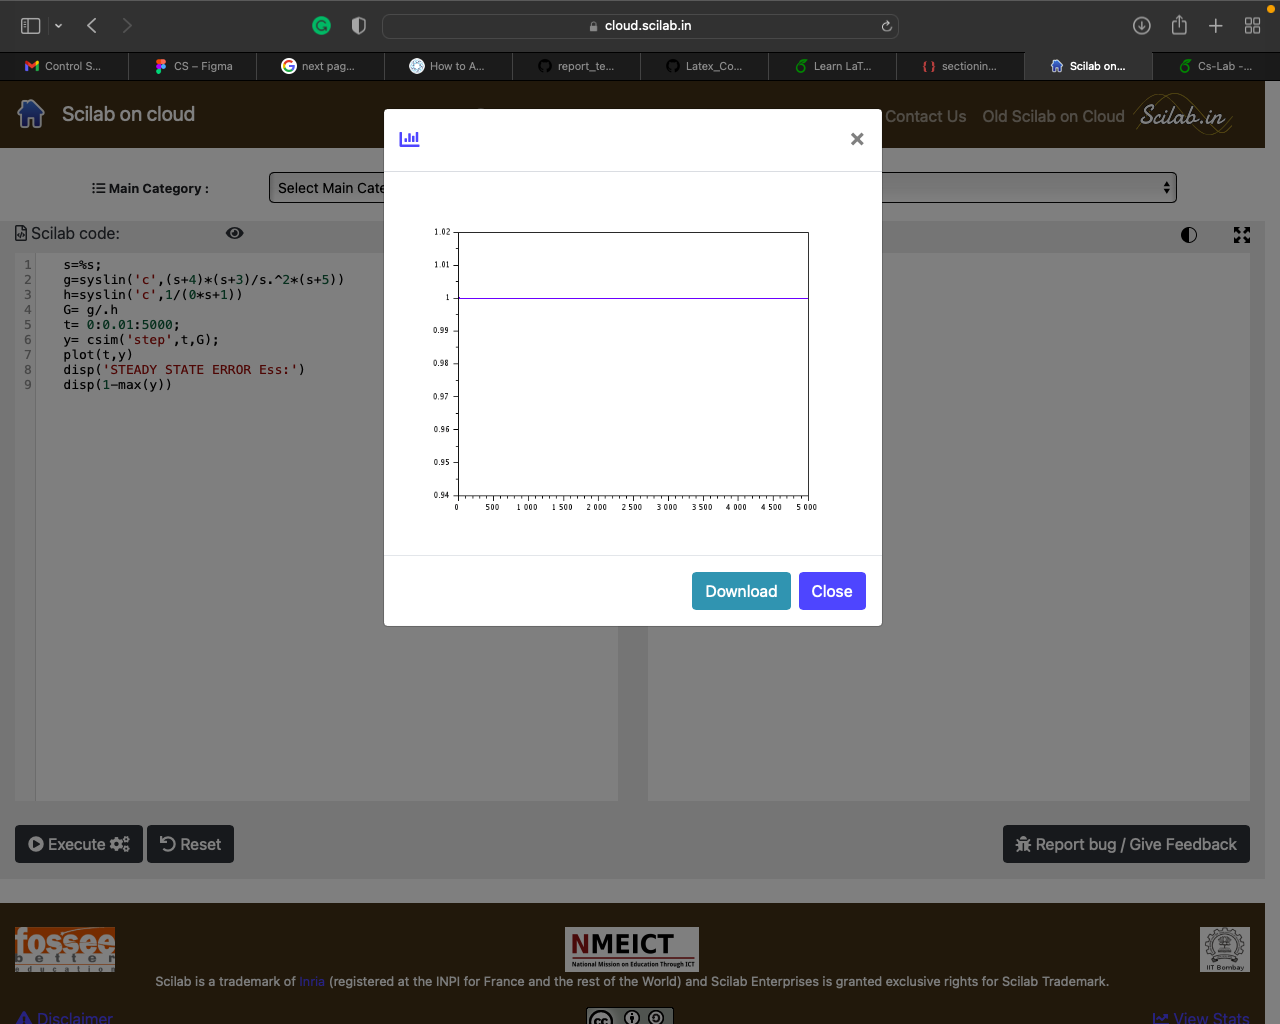
\includegraphics[width =10cm, height = 10cm]{images/exp71.png}
        \caption{Graph}
        \label{Graph}
\end{figure}
\begin{figure}[!hth]
        \centering
        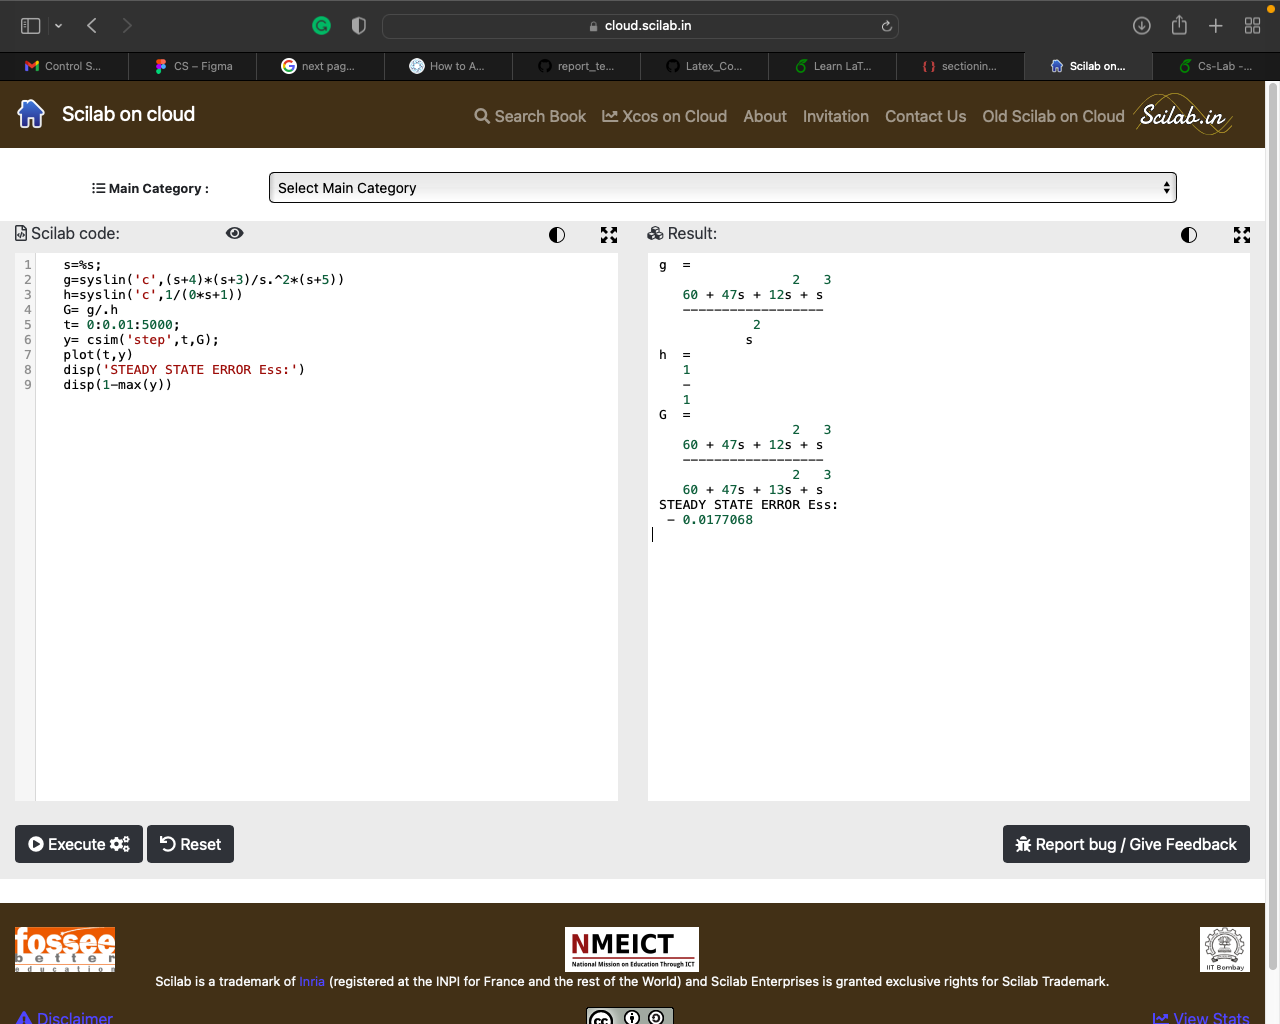
\includegraphics[width =10cm, height = 10cm]{images/exp72.png}
        \caption{Result}
        \label{Result}
\end{figure}

\section*{\textcolor{black}{Conclusion}}
 We get zero difference i.e zero error for step input in type 2 as we increase the time.
    \pagebreak
\maketitle
\begin{center}
    \LARGE {EXPERIMENT NO : 8}
             
\end{center}

\section*{\textcolor{black}{AIM: }}
\text{To calculate steady state error in velocity of Type 2}

\section*{\textcolor{black}{Block Diagram :}}

\begin{figure}[!hth]
        \centering
        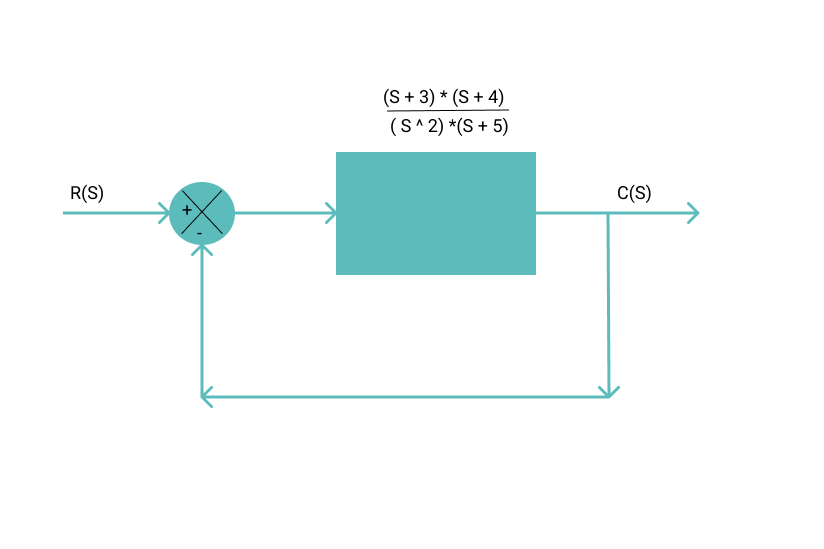
\includegraphics[width =10cm, height = 7cm]{images/exp8.png}
        \caption{Block Diagram}
        \label{Graph}
\end{figure}

\section*{\textcolor{black}{Theory :}}
Steady-state error is defined as the difference between the desired value and the actual value of a system output in the limit as time goes to infinity (i.e. when the response of the control system has reached steady-state).\par

Steady-state error is a property of the input/output response for a linear system. In general, a good control system will be one that has a low steady-state error
For a Type 0 system, the error is a non-zero, finite number, and Kp is equal to the Bode gain Kx. \par

\section*{\textcolor{black}{Code :}}

   s=\%s;\\ 
   g=syslin('c',(s+4)(s+3)/s.\wedge2(s+5))\\
   h=syslin('c',1/(0*s+1))\\
   G= g/.h\\
   t= 0:0.01:5;\\
   y= csim(t,t,G);\\
   plot(t,y)\\
    plot(t,t,'red')\\
   disp('STEADY STATE ERROR Ess:')\\
   disp(max(t)-max(y)) \par 

\section*{\textcolor{black}{OUTPUT/OBSERVATIONS}}

\begin{figure}[!hth]
        \centering
        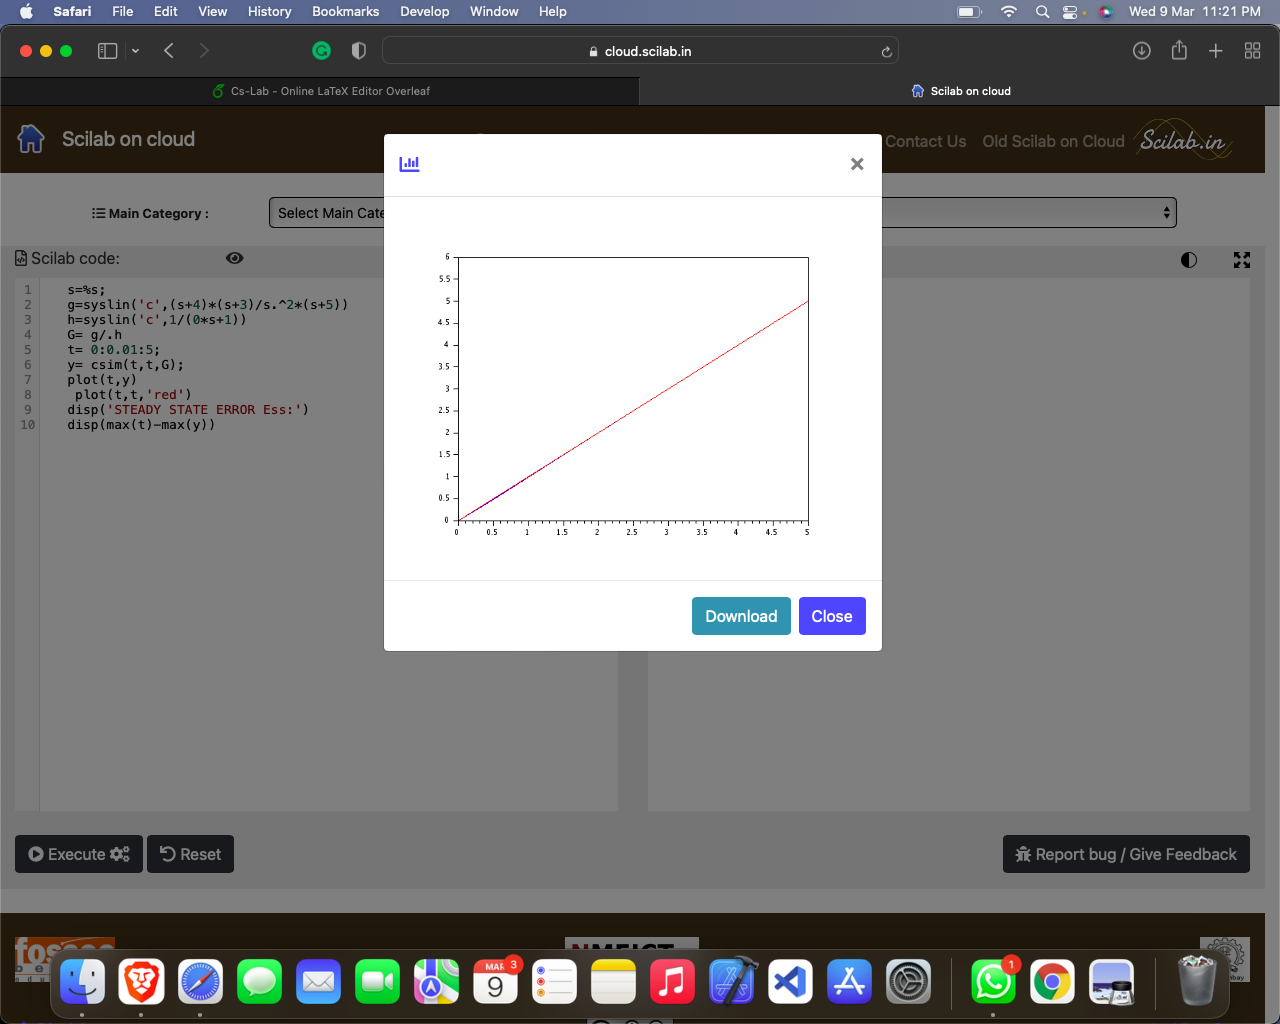
\includegraphics[width =10cm, height = 10cm]{images/exp81.png}
        \caption{Graph}
        \label{Graph}
\end{figure}
\begin{figure}[!hth]
        \centering
        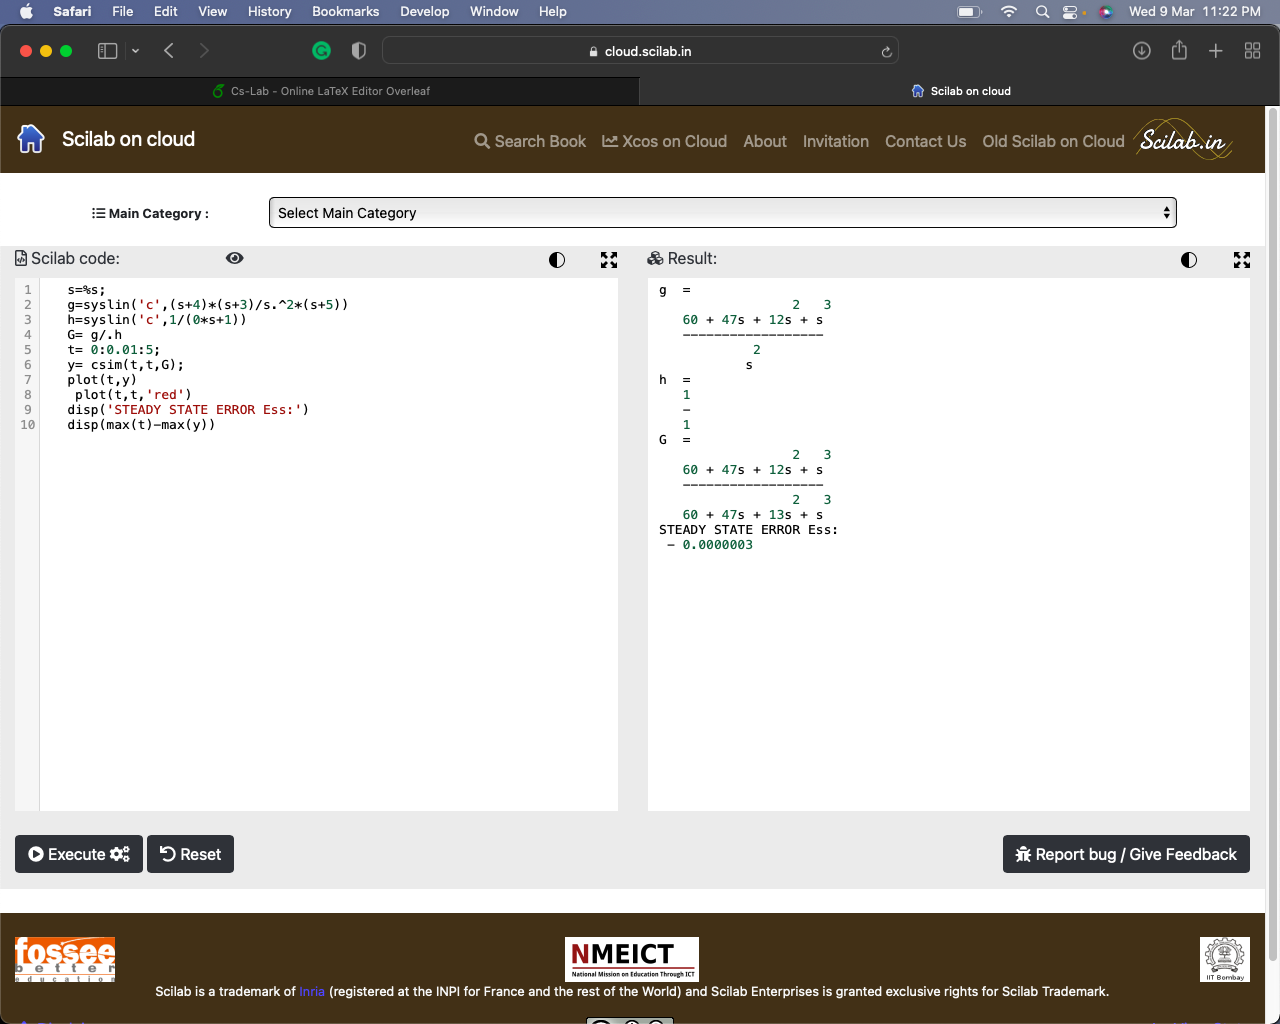
\includegraphics[width =10cm, height = 10cm]{images/exp82.png}
        \caption{Result}
        \label{Result}
\end{figure}

\section*{\textcolor{black}{Conclusion}}
 When we give a ramp input to type 2 system then we get 0 error as we increase the time.
     \pagebreak
\maketitle
\begin{center}
    \LARGE {EXPERIMENT NO : 9}
             
\end{center}

\section*{\textcolor{black}{AIM: }}
\text{To calculate steady state error in acceleration of Type 2}

\section*{\textcolor{black}{Block Diagram :}}

\begin{figure}[!hth]
        \centering
        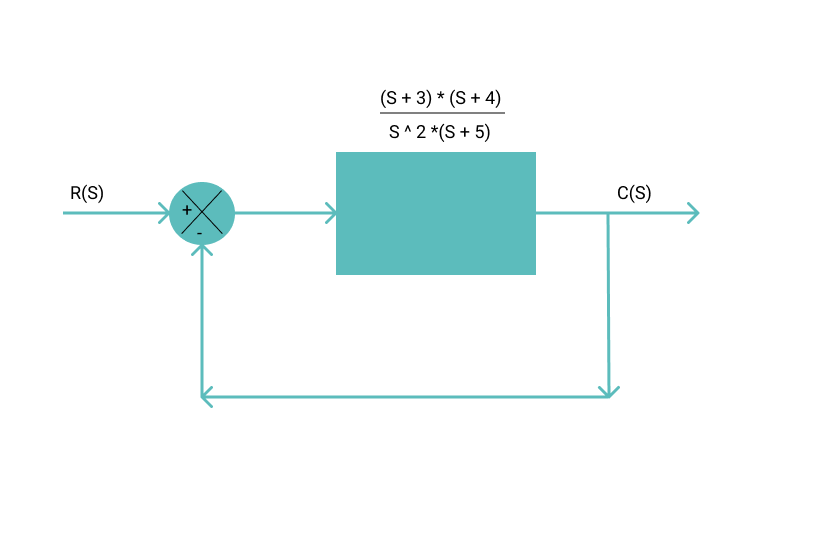
\includegraphics[width =10cm, height = 7cm]{images/exp9.png}
        \caption{Block Diagram}
        \label{Graph}
\end{figure}


\section*{\textcolor{black}{Theory :}}
Steady-state error is defined as the difference between the desired value and the actual value of a system output in the limit as time goes to infinity (i.e. when the response of the control system has reached steady-state).\par

Steady-state error is a property of the input/output response for a linear system. In general, a good control system will be one that has a low steady-state error
For a Type 0 system, the error is a non-zero, finite number, and Kp is equal to the Bode gain Kx. \par

\section*{\textcolor{black}{Code :}}

   s=\%s;\\ 
   g=syslin('c',(s+4)(s+3)/s.\wedge2(s+5))\\
   h=syslin('c',1/(0*s+1))\\
   G= g/.h\\
   t= 0:0.01:5;\\
   y= csim(t.\wedge2,t,G);\\
   plot(t,y)\\
    plot(t,t.\wedge2,'red')\\
   disp('STEADY STATE ERROR Ess:')\\
   disp(max(t.\wedge2)-max(y)) \par 

\section*{\textcolor{black}{OUTPUT/OBSERVATIONS}}

\begin{figure}[!hth]
        \centering
        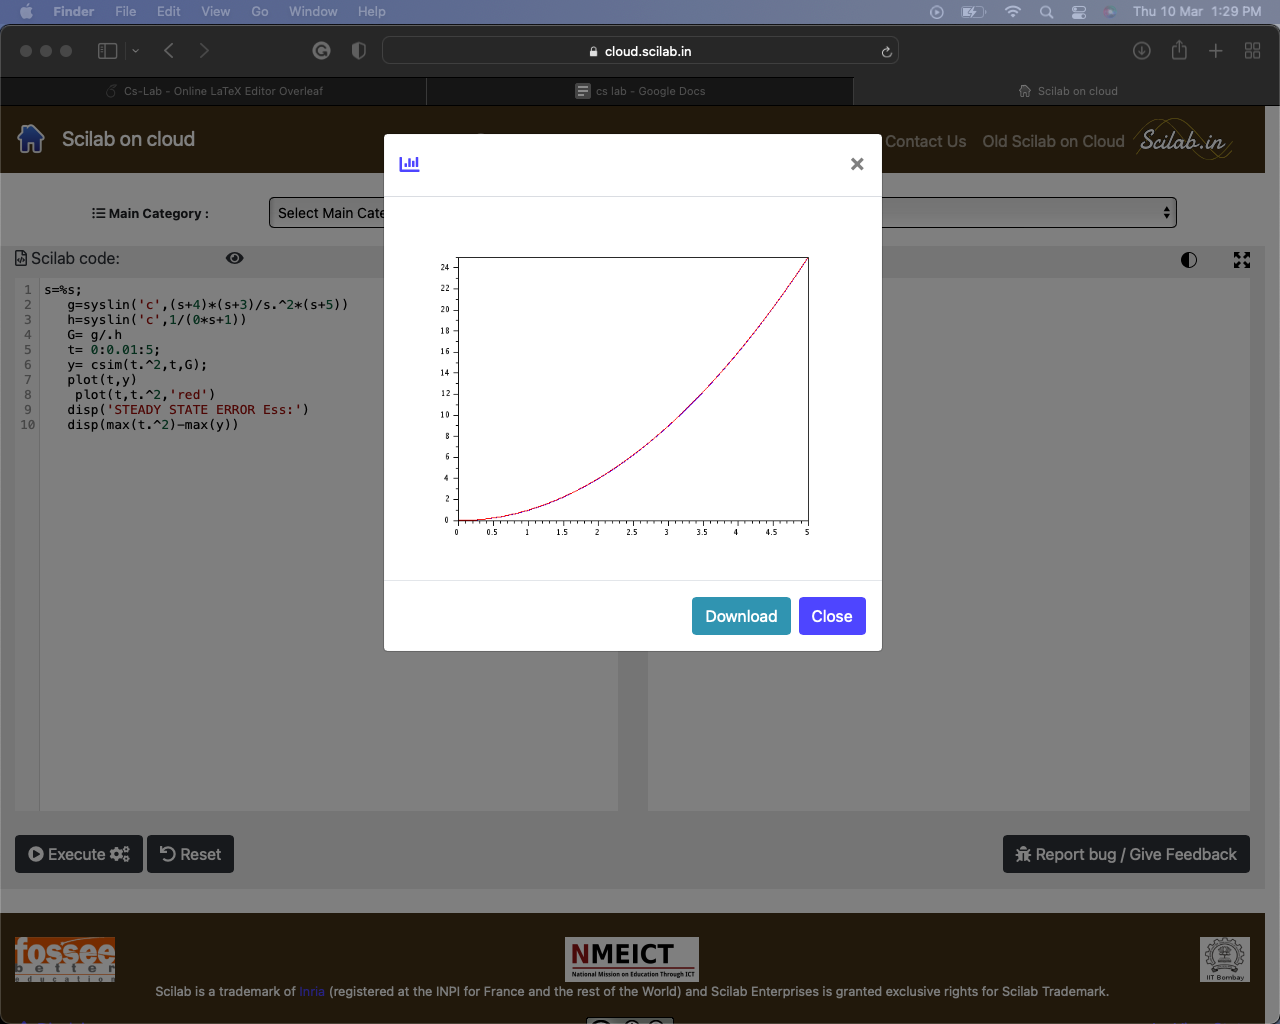
\includegraphics[width =10cm, height = 10cm]{images/exp91.png}
        \caption{Graph}
        \label{Graph}
\end{figure}
\begin{figure}[!hth]
        \centering
        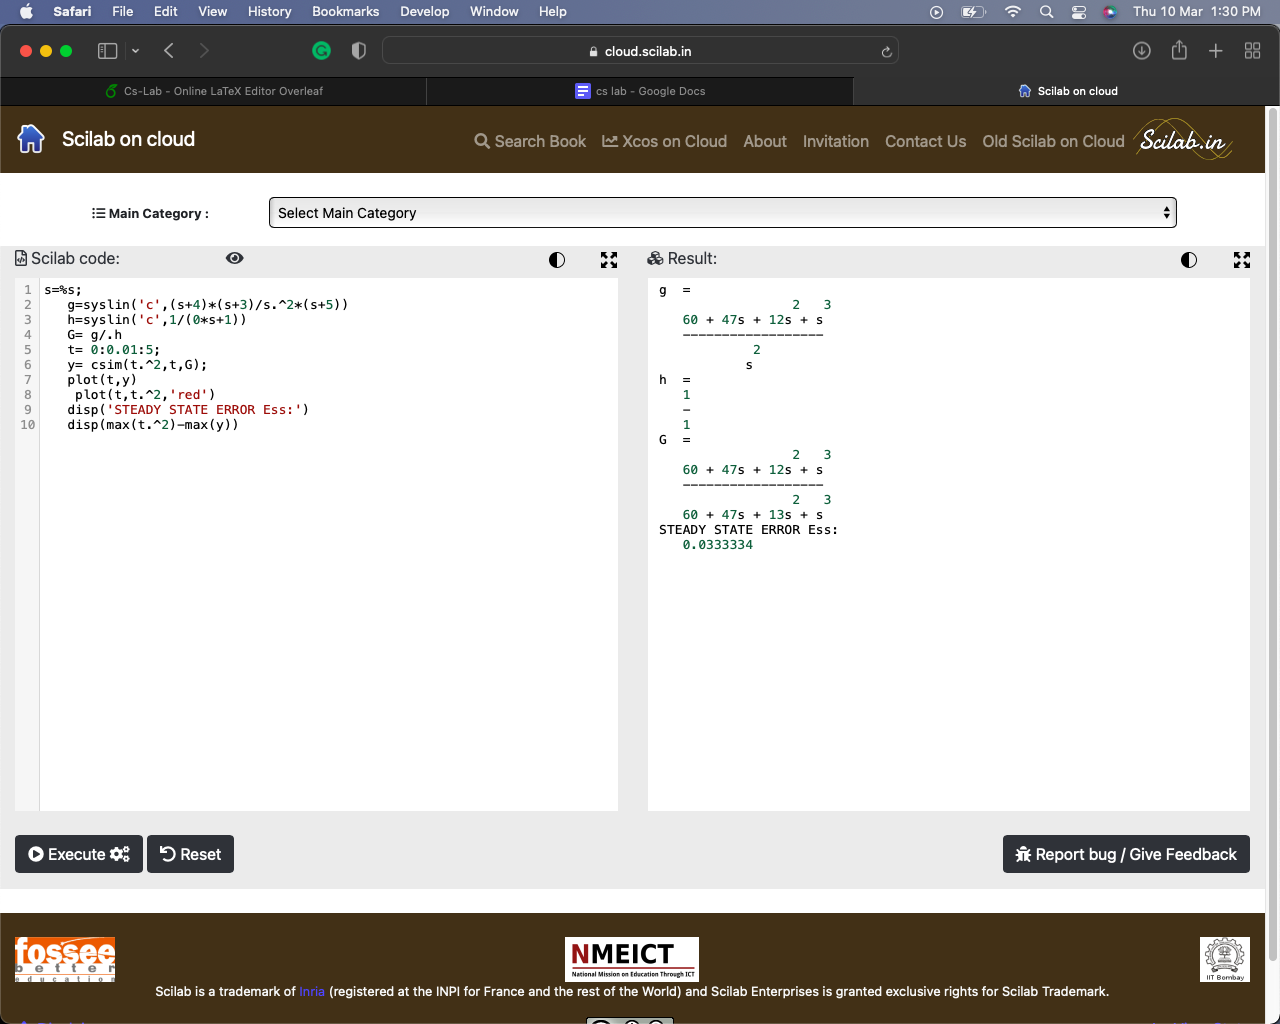
\includegraphics[width =10cm, height = 10cm]{images/exp92.png}
        \caption{Result}
        \label{Result}
\end{figure}

\section*{\textcolor{black}{Conclusion}}
After giving a parabolic input to type 2 system we get a constant error which is equal to 1/Ka.
 
 \pagebreak
 \begin{center}
    \LARGE {EXPERIMENT NO : 10}
             
\end{center}

\section*{\textcolor{black}{AIM:}}
\text{Calculating Transfer Function of Block Diagram by Reduction }

\section*{\textcolor{black}{Block Diagram :}}

\begin{figure}[!hth]
        \centering
        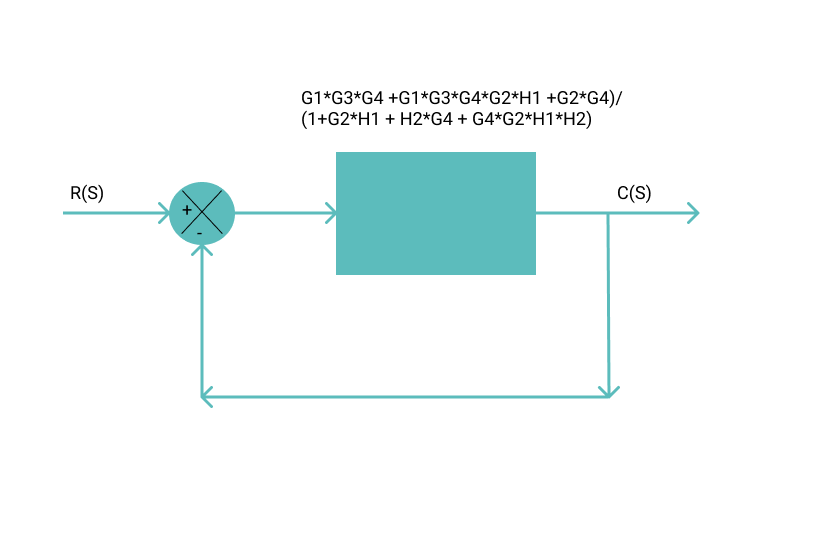
\includegraphics[width =10cm, height = 7cm]{images/Transfer funstion.png}
        \caption{Block Diagram}
        \label{Graph}
\end{figure}

\section*{\textcolor{black}{Theory :}}The gains in series are multiplied. And gain having a feedback having G(S) and H(s) is feedback gain .The combined value is given by $ G(S)/(1+H(S)*G(S)) $
 \par

\section*{\textcolor{black}{Code :}}
s=\%s;\\
g1= 10/(0*s +1);\\
G1 = syslin('c', g1);\\
g2=1/(s);\\
G2 = syslin('c', g2);\\
g3 = 1/(s+5);\\
G3 = syslin('c', g3);\\
g4= 2*s/(0*s+1);\\
G4 = syslin('c', g4);\\
h1 = 1/(s*0+1);\\
H1= syslin('c',h1);\\
h2= 1/s;\\
H2= syslin('c',h2);\\
//computing transfer function
Tmanual= (G1*G3*G4 +G1*G3*G4*G2*H1 +G2*G4)/(1+G2*H1 + H2*G4 + G4*G2*H1*H2);\\
disp('manually computed');\\
disp(Tmanual);\\
//computing using built-in commands
sub1=G1*G3;\\
sub2 = G2/.H1;\\
sub3 = G4/.H2;\\
sub4 = sub1 + sub2;\\
Tauto= sub4*sub3;\\
disp('auto computed');\\
disp(Tauto);\\ \par 

\section*{\textcolor{black}{OUTPUT/OBSERVATIONS}}

\begin{figure}[!hth]
        \centering
        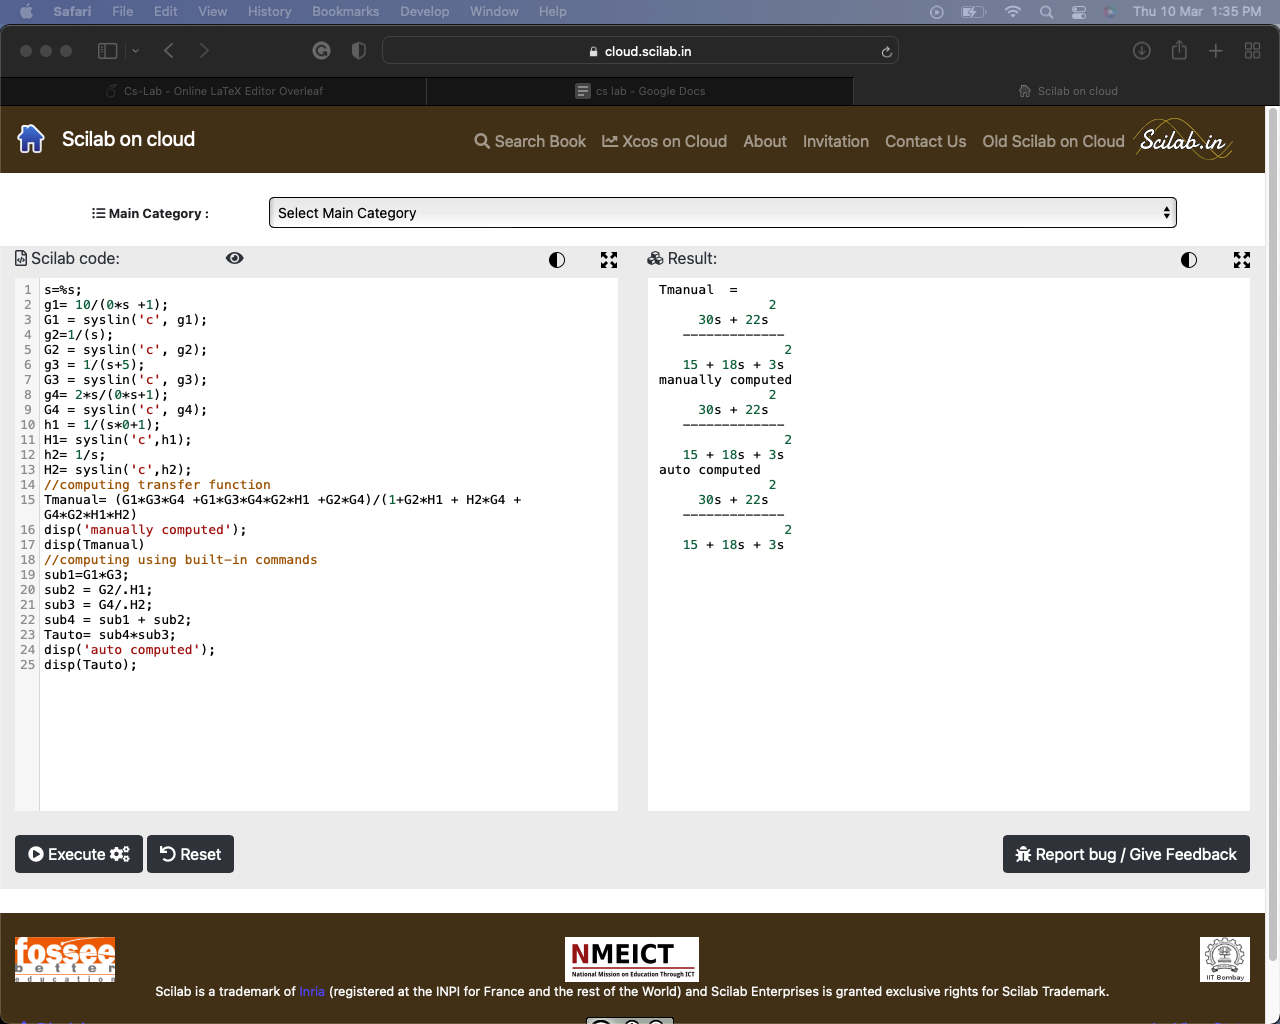
\includegraphics[width =10cm, height = 10cm]{images/exp101.png}
        \caption{Result}
        \label{Result}
\end{figure}


\section*{\textcolor{black}{Conclusion}}
It can be concluded that for complex block structures, block reduction tech- niques can be used to simplify the calculation and find our results without any error creeping in in our calculations.
 \pagebreak

 \begin{center}
    \LARGE {EXPERIMENT NO : 11}
             
\end{center}

\section*{\textcolor{black}{AIM: }}
\text{Speed Control in DC Motor}


\section*{\textcolor{black}{Block Diagram :}}

\begin{figure}[!hth]
        \centering
        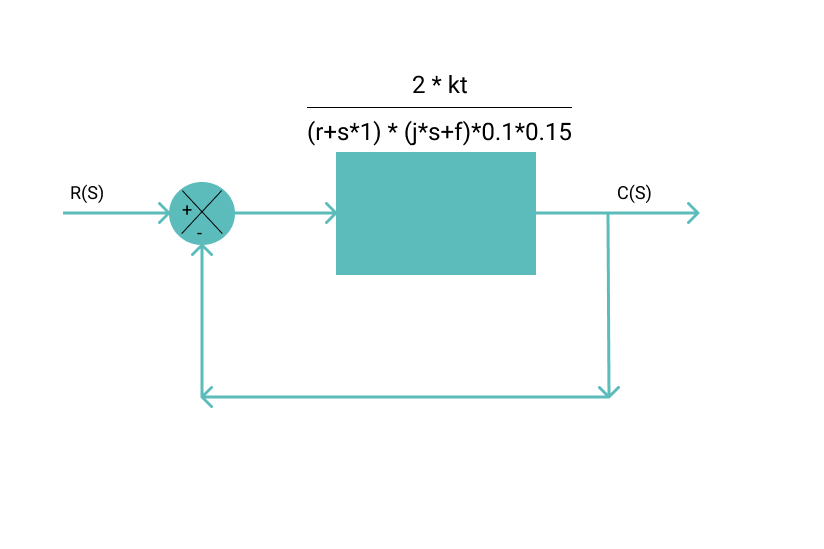
\includegraphics[width =10cm, height = 7cm]{images/speed control.png}
        \caption{Block Diagram}
        \label{Graph}
\end{figure}

\section*{\textcolor{black}{Theory :}}
We can control the speed of DC motor manually or through an automatic control device. This is different to speed regulation – where the speed can regulate against the natural change in speed due to a change in the load on the shaft.The speed of a DC motor (N) is equal to
N = K (V – IaRa)/ ø Where, K is a constant.

Thus, the speed of a DC motor can control in three ways;

-By varying the flux, and by varying the current through field winding
-By varying the armature voltage, and the armature resistance
-Through the supply voltage   
 \par

\section*{\textcolor{black}{Code :}}

  r=2;\\
l=0.5;\\
kt=0.1;   //magnetic flux\\
kb=0.1;\\
f=0.2;\\
j=0.02;\\
ka=2;       //f\\
ktm=0.15;  //feedback\\
 
s=\%s;\\
v2i=syslin('c',1/(r+s*1))\\
i2w=syslin('c',kt/(j*s+f))\\

dcm=v2i*i2w/.kb\\
tf=(ka*dcm)/.ktm\\
t=0:0.01:2;\\
ystep=csim('impulse',t,tf);\\

plot(t,ystep) \\\par 

\section*{\textcolor{black}{OUTPUT/OBSERVATIONS}}

\begin{figure}[!hth]
        \centering
        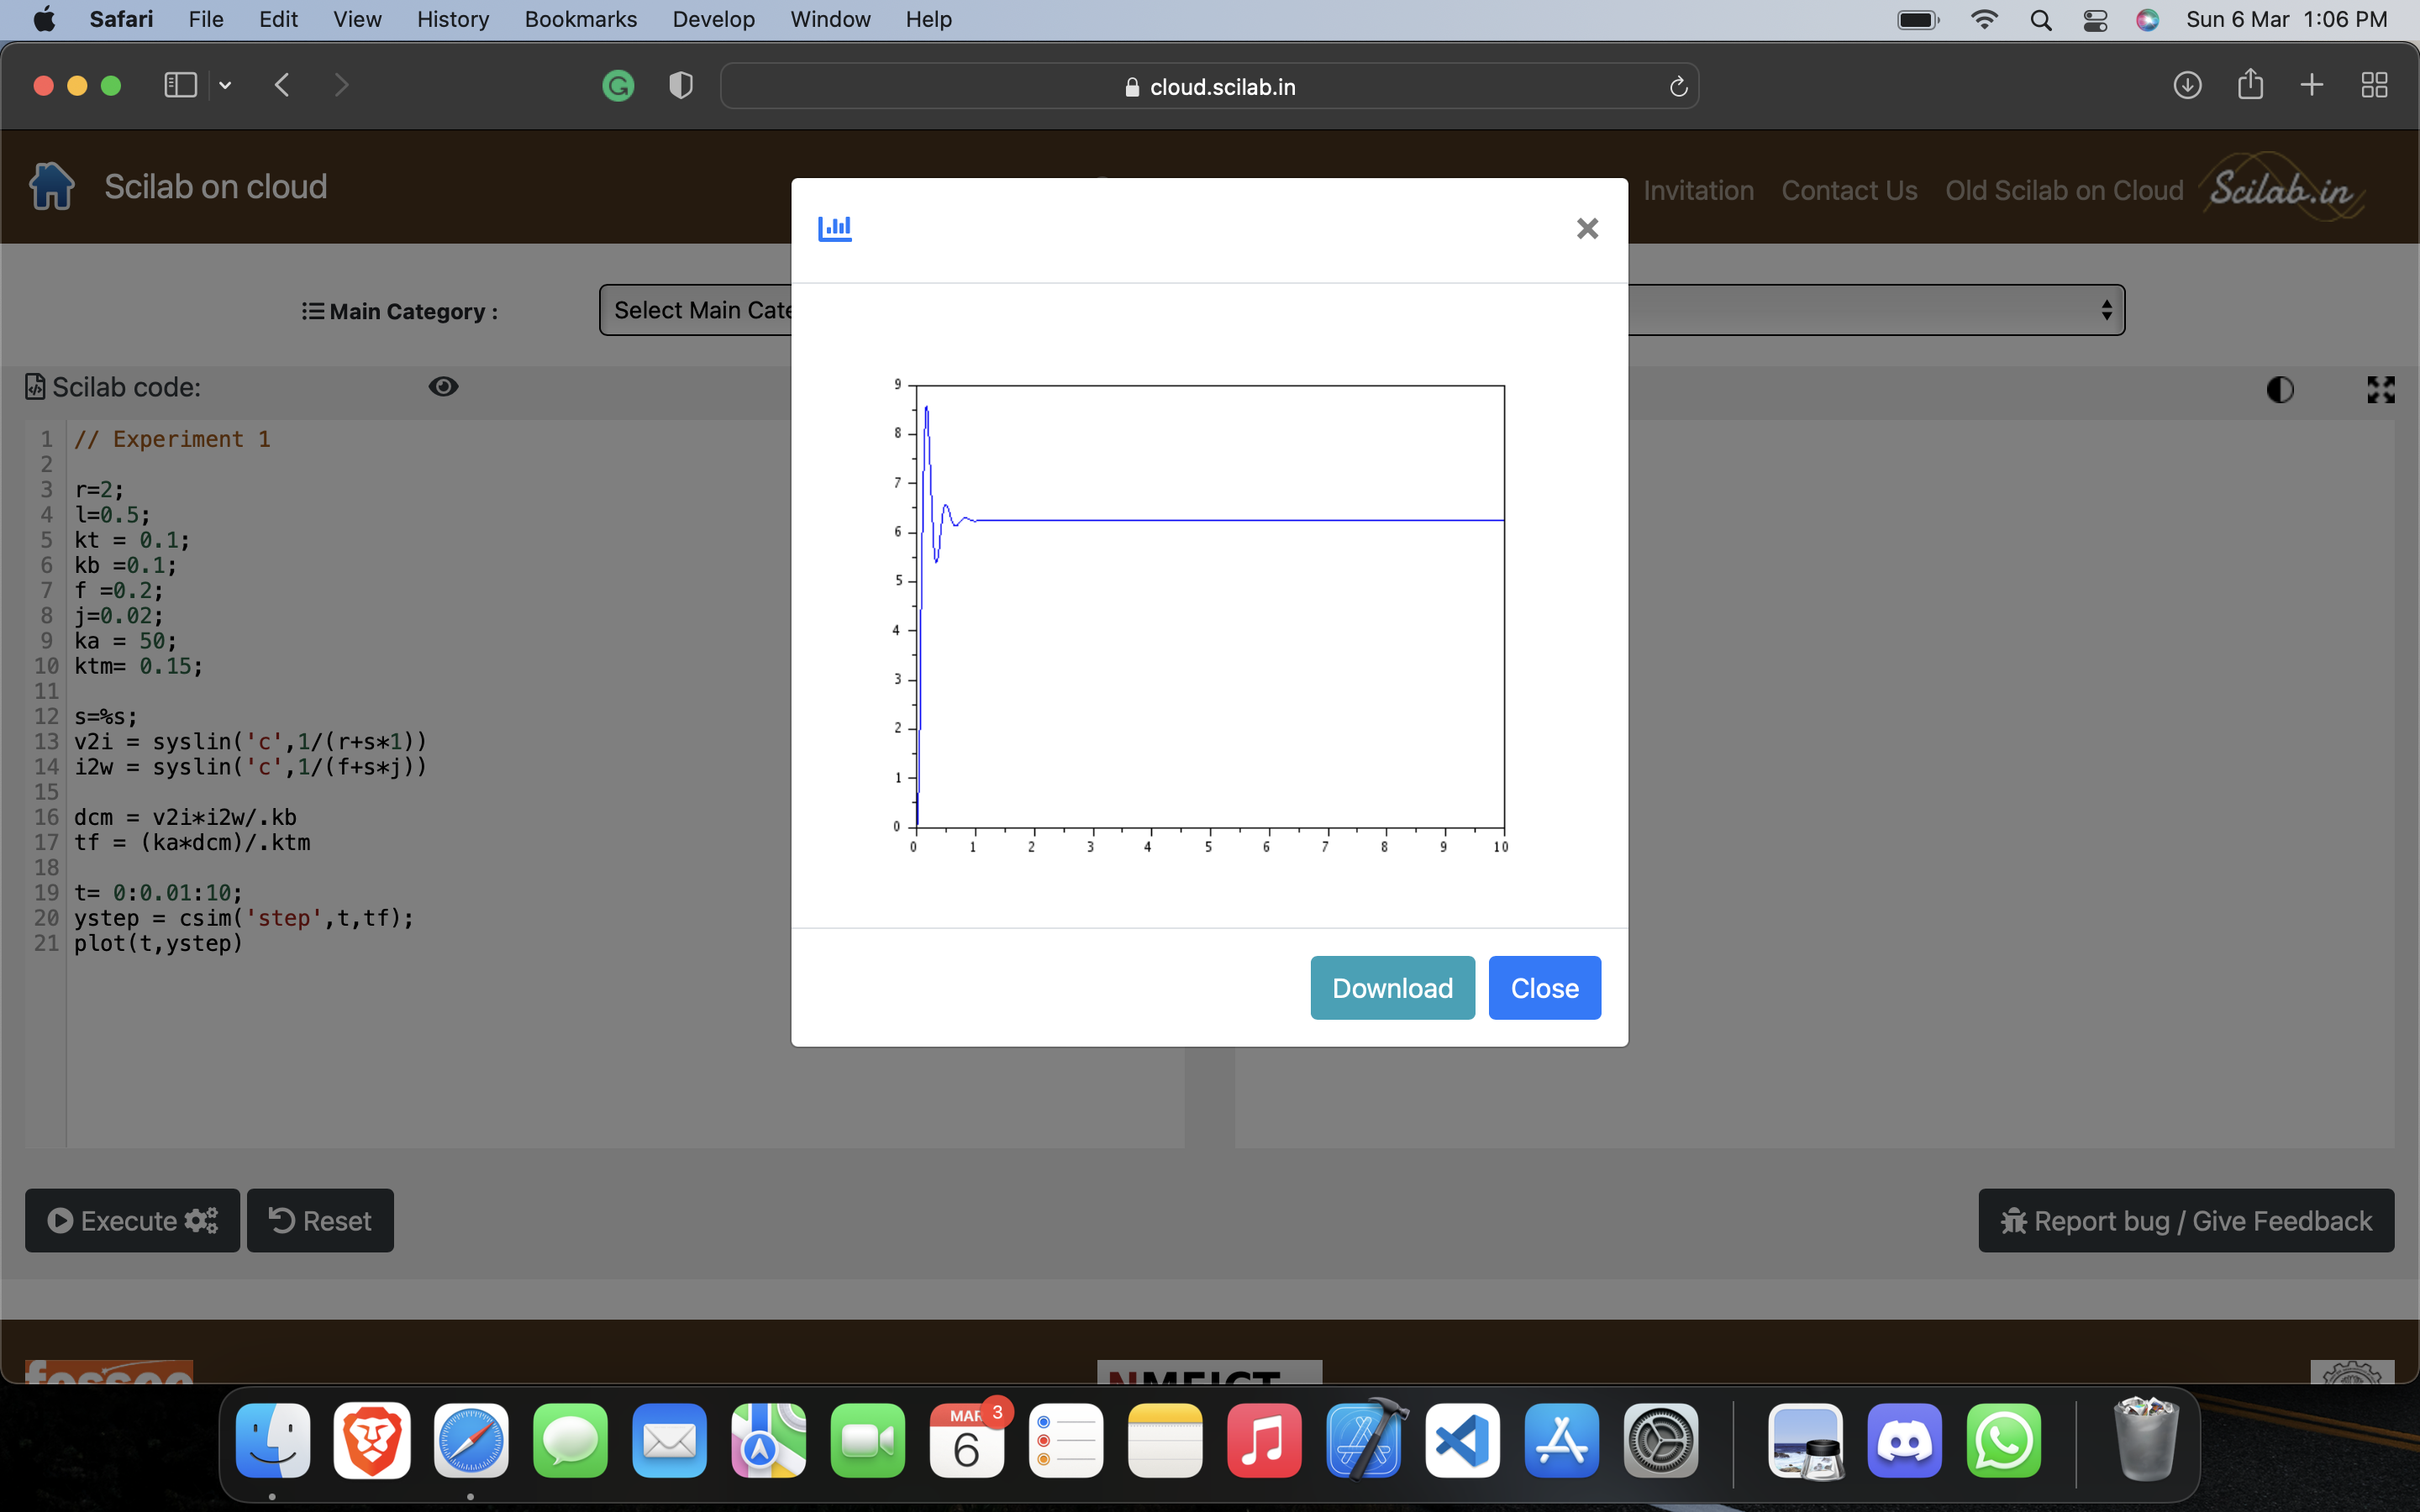
\includegraphics[width =10cm, height = 10cm]{images/Experiment1-output..png}
        \caption{Graph}
        \label{Graph}
\end{figure}
\begin{figure}[!hth]
        \centering
        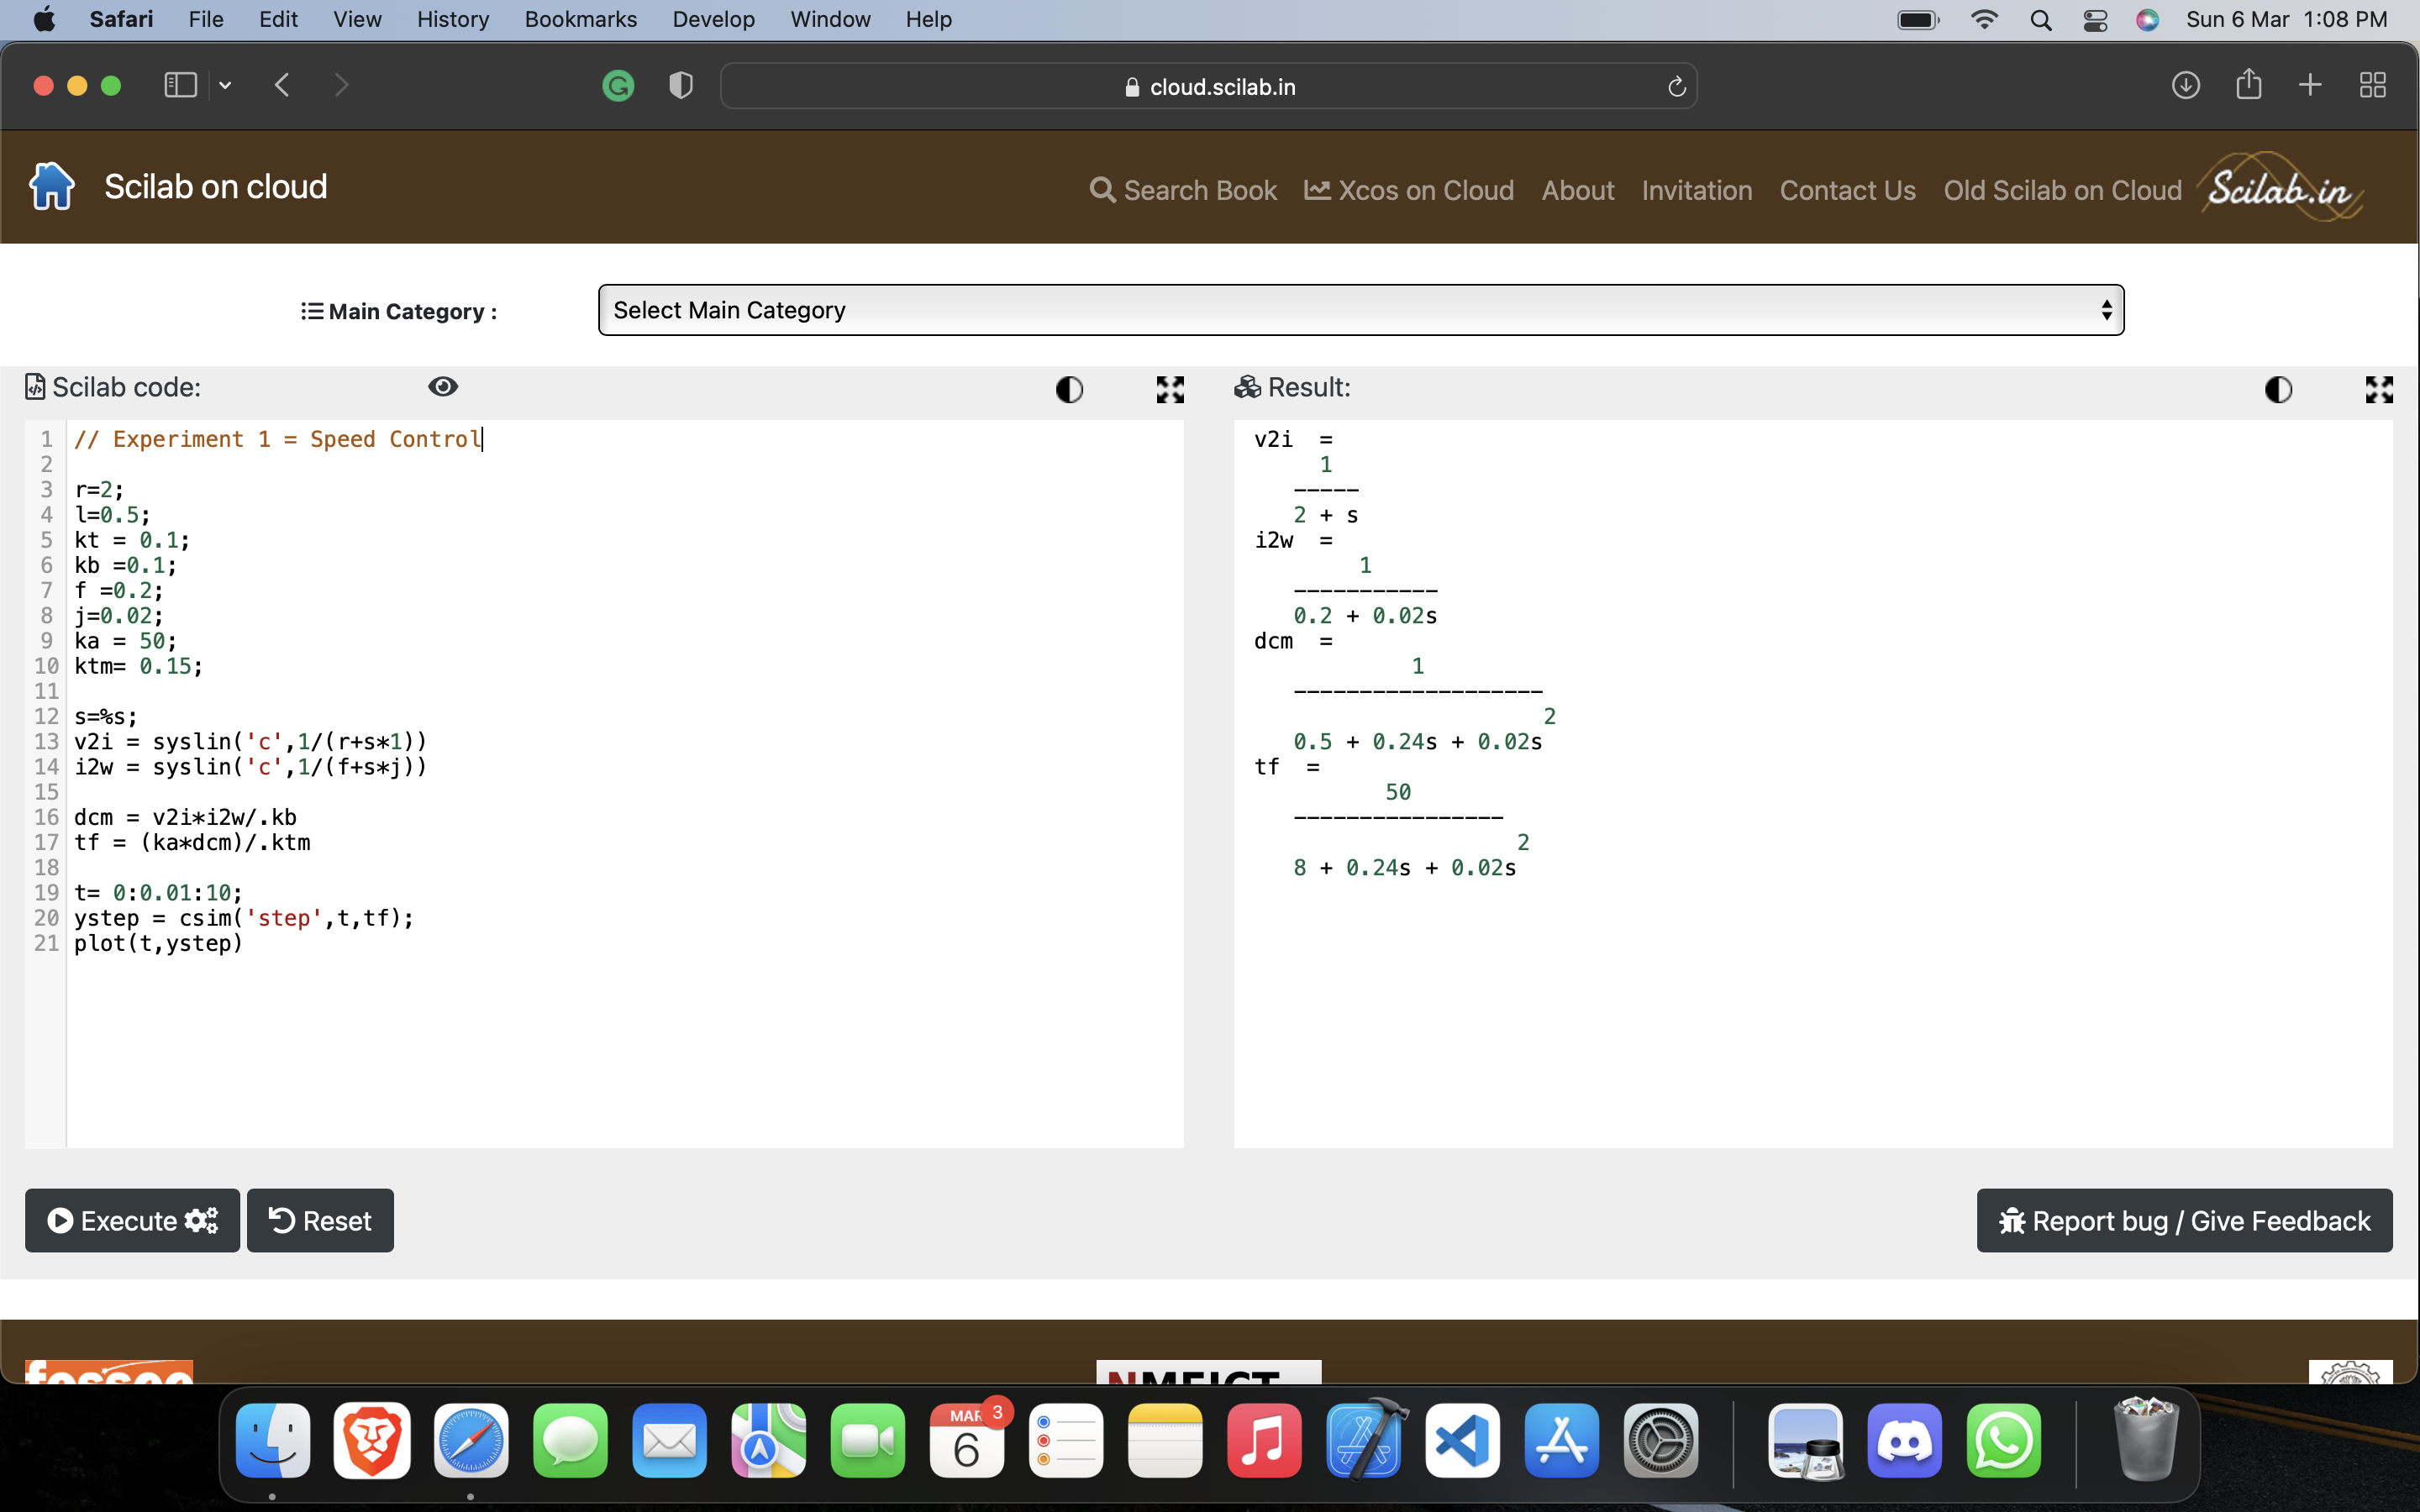
\includegraphics[width =10cm, height = 10cm]{images/Experiment1.png}
        \caption{Result}
        \label{Result}
\end{figure}

\section*{\textcolor{black}{Conclusion}}
From the above experiment, it can be concluded that various real world control systems can be realised and carefully calculated using control system tools. The speed control system of a motor can particularly be realised and its movements can be calculated by considering it as a second order system.
      
\pagebreak

\begin{center}
    \LARGE {EXPERIMENT NO : 12}
             
\end{center}

\section*{\textcolor{black}{AIM:}}
\text{Plotting Damping Factor and Wn values}

\section*{\textcolor{black}{Block Diagram :}}

\begin{figure}[!hth]
        \centering
        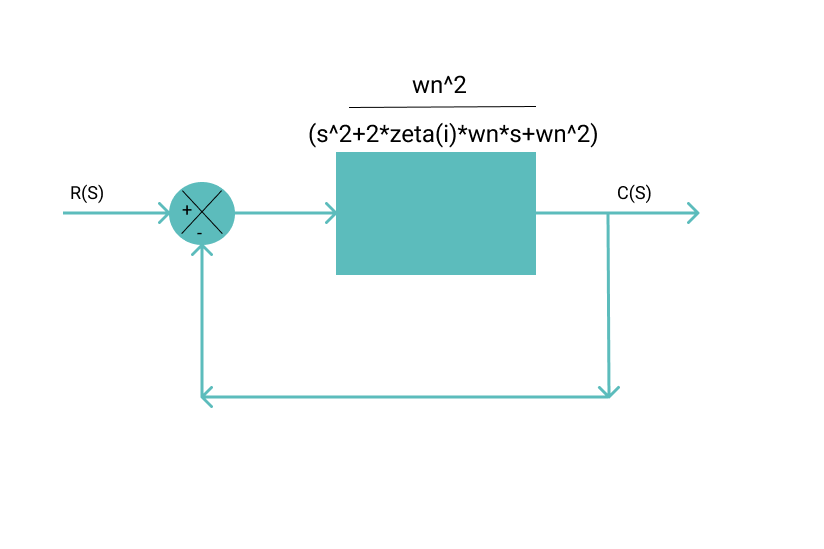
\includegraphics[width =10cm, height = 7cm]{images/damping factor.png}
        \caption{Block Diagram}
        \label{Graph}
\end{figure}

\section*{\textcolor{black}{Theory :}}
Plotting 2nd Order Time Response for different zeta values and a natural frequency value.Damping factor:
The damping ratio is defined as the number of oscillations in a system that can decay or restrain after an interruption and it is a dimensionless measurement. Most of the systems work in oscillatory mode when they are interrupted or disturbed from their initial position. For example, suspension of mass from a spring. If the mass is pulled and released, then it bounces up and down. The system tries to return to its initial static position after every bounce.
The damping ratio symbol is denoted as ‘ζ’ (Zeta).\par

\section*{\textcolor{black}{Code :}}
s= \%s;\\
zeta= [0 0.2 0.5 1 5 20];\\
wn=10;\\
col = ['r' 'b' 'g' 'b' 'r' 'g']\\
for i=1:6\\
     G=syslin('c',wn\wedge2/(s\wedge2+2*zeta(i)*wn*s+wn\wedge2))\\
     t=0:0.01:5;\\
     ystep=csim('step',t,G);\\
     plot(t,ystep,col(i));\\
end\\
   \par 

\section*{\textcolor{black}{OUTPUT/OBSERVATIONS}}

\begin{figure}[!hth]
        \centering
        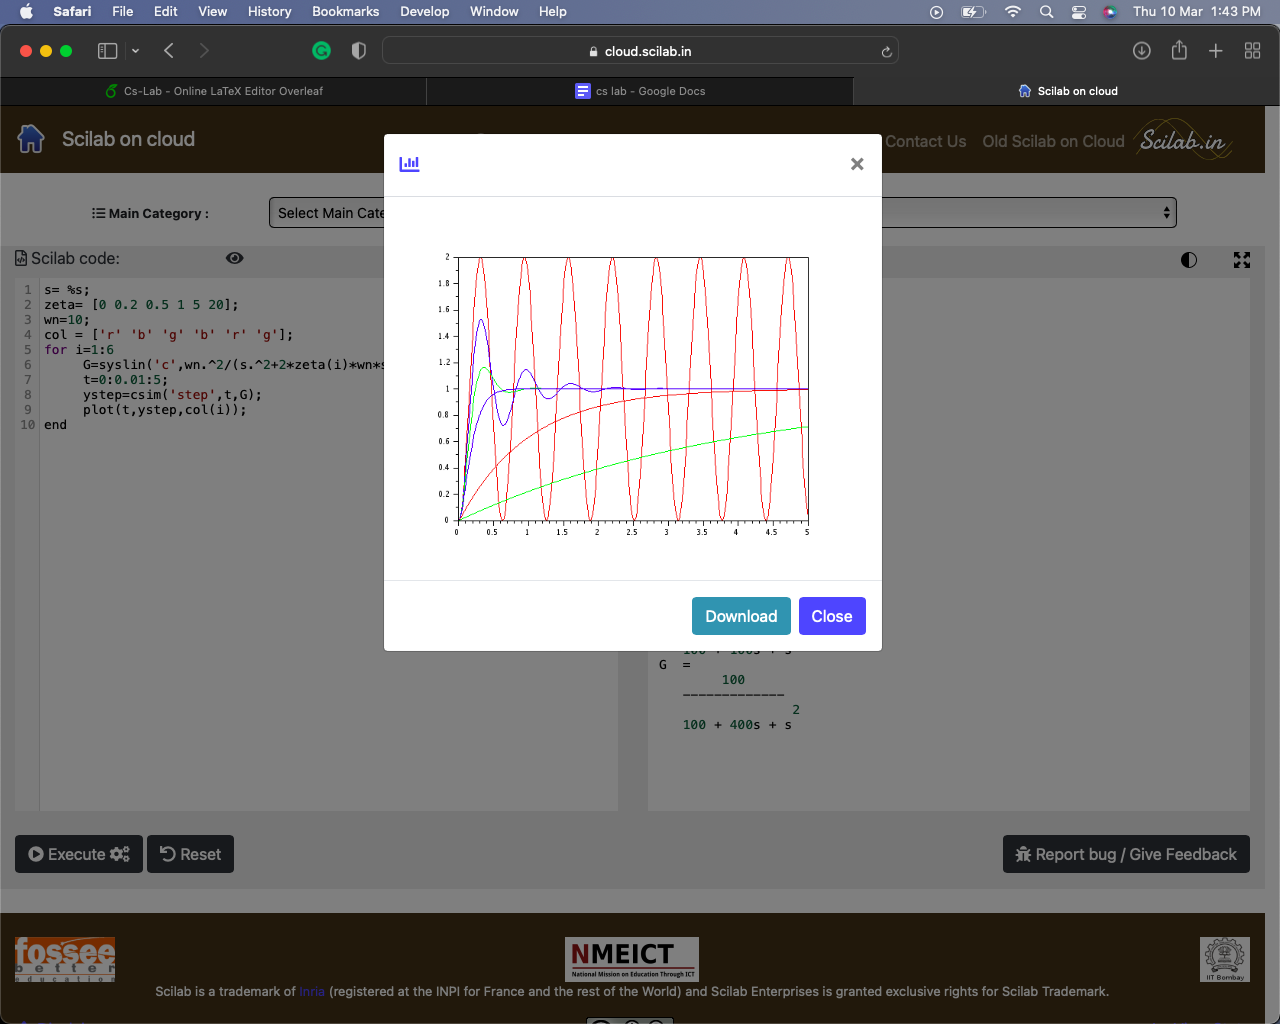
\includegraphics[width =10cm, height = 10cm]{images/exp121.png}
        \caption{Graph}
        \label{Graph}
\end{figure}
\begin{figure}[!hth]
        \centering
        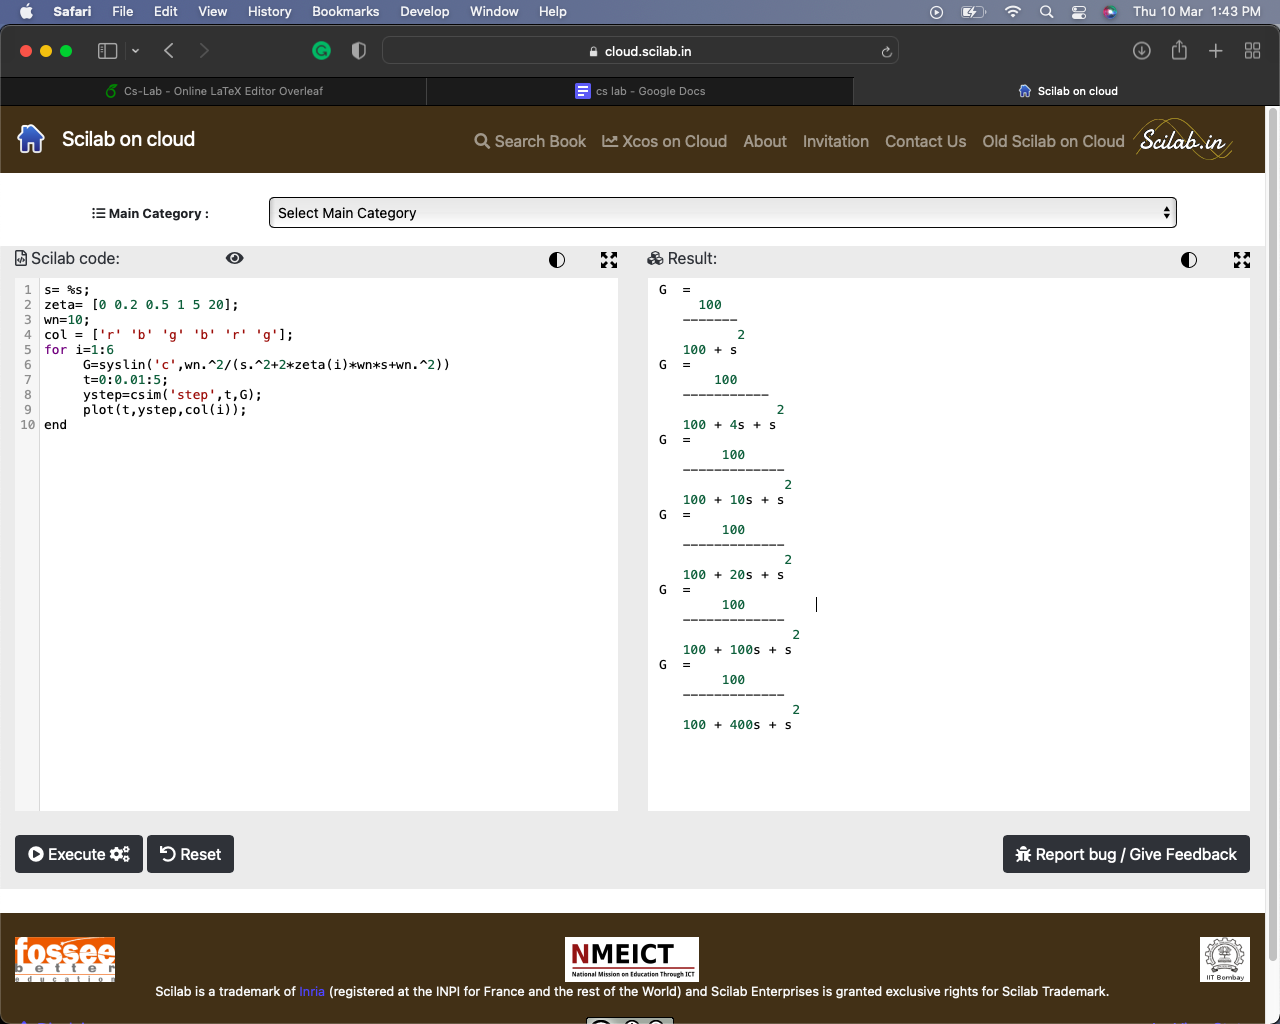
\includegraphics[width =10cm, height = 10cm]{images/exp122.png}
        \caption{Result}
        \label{Result}
\end{figure}

\section*{\textcolor{black}{Conclusion}}
From the above experiment, it can be concluded that for getting a desired output, we should consider the value of zeta between zero and one. This way, we get our system output in less time with few inconsistencies in the beginning.
 \pagebreak

\begin{center}
    \LARGE {EXPERIMENT NO : 13}
             
\end{center}

\section*{\textcolor{black}{AIM: }}
\text{Plot poles using different zeta values}

\section*{\textcolor{black}{Block Diagram :}}

\begin{figure}[!hth]
        \centering
        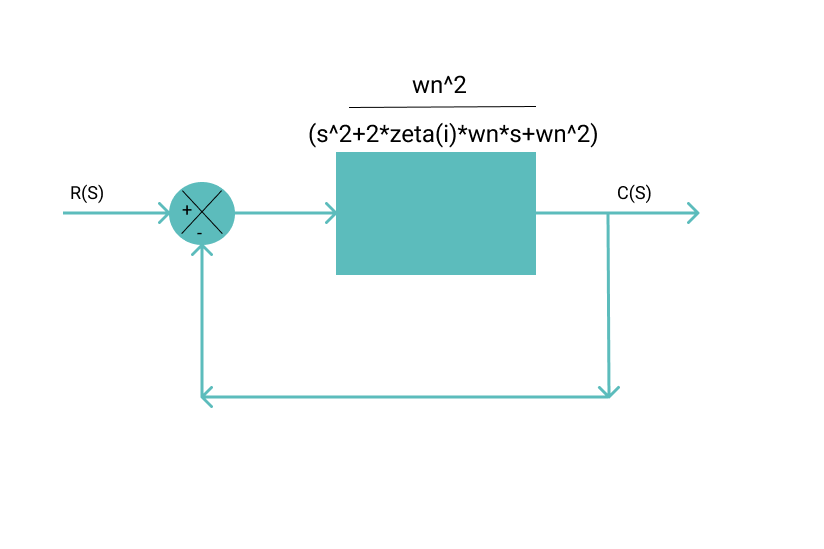
\includegraphics[width =10cm, height = 7cm]{images/damping factor.png}
        \caption{Block Diagram}
        \label{Graph}
\end{figure}

\section*{\textcolor{black}{Theory :}}
POLES:The values for which the equation in denominator for a transfer function is Zero.
 Zeta = Damping factor of 2nd order Time Response 
  wn =natural frequency.
zeta — Damping ratio of each pole
Damping ratios of each pole, returned as a vector sorted in the same order as wn .If sys is a discrete-time model with specified sample time, zeta contains the damping ratios of the equivalent continuous-time poles
 \par

\section*{\textcolor{black}{Code :}}
s= \%s;\ 
zeta= [0 0.2 0.5 1 5 20];\\
wn=10;\\
col = ['r' 'b' 'g' 'b' 'r' 'g']\\
for i=1:6\\
     G=syslin('c',(wn)\wedge2/(s\wedge2+2*zeta(i)*wn*s+(wn)\wedge2))\\
     plzr(G)\\
end\\

   \par 

\section*{\textcolor{black}{OUTPUT/OBSERVATIONS}}

\begin{figure}[!hth]
        \centering
        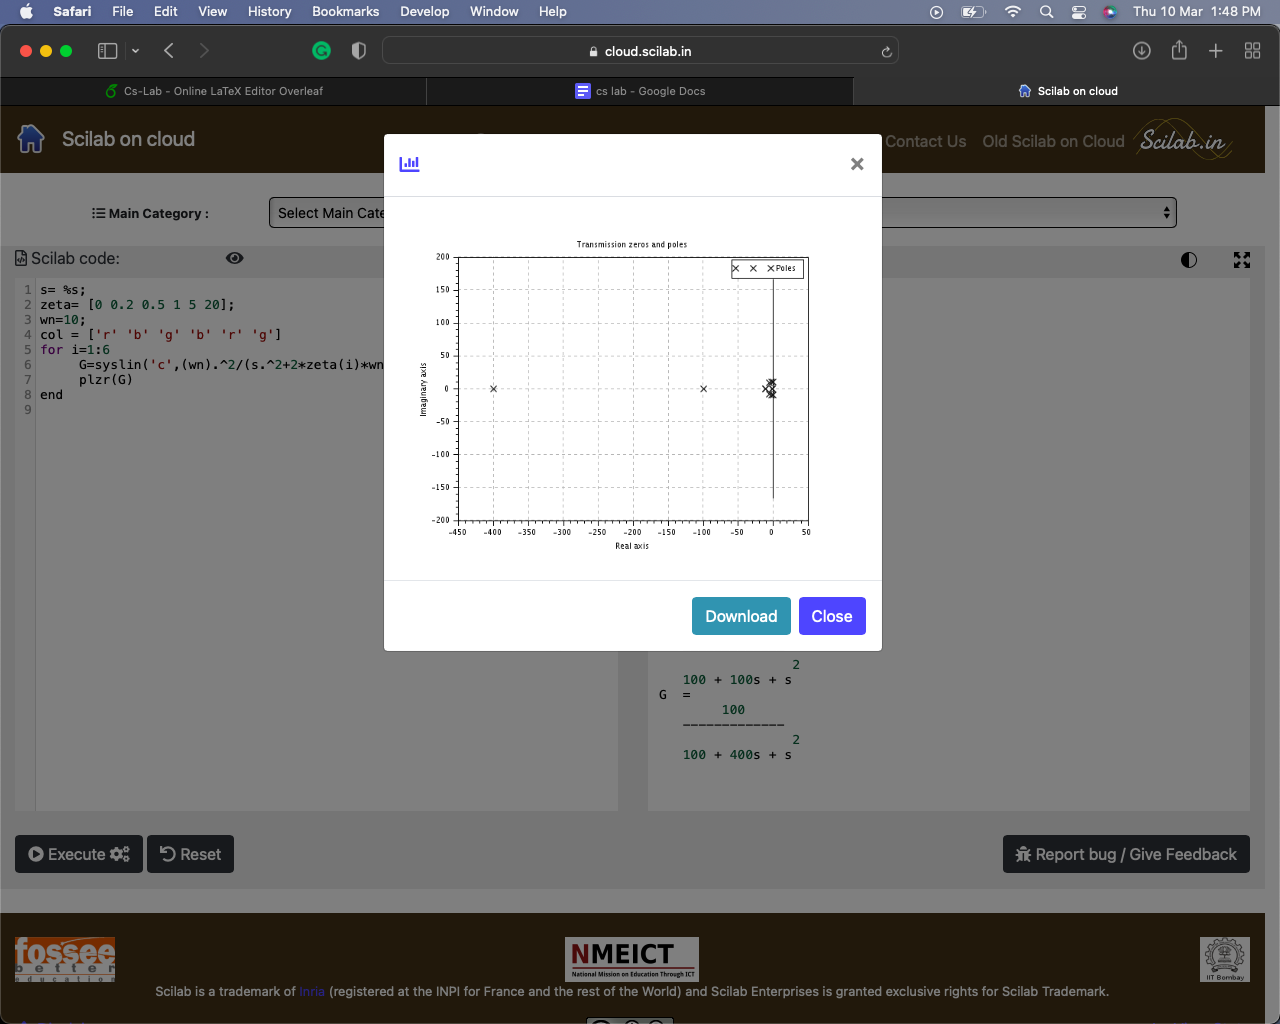
\includegraphics[width =10cm, height = 10cm]{images/exp131.png}
        \caption{Graph}
        \label{Graph}
\end{figure}

\begin{figure}[!hth]
        \centering
        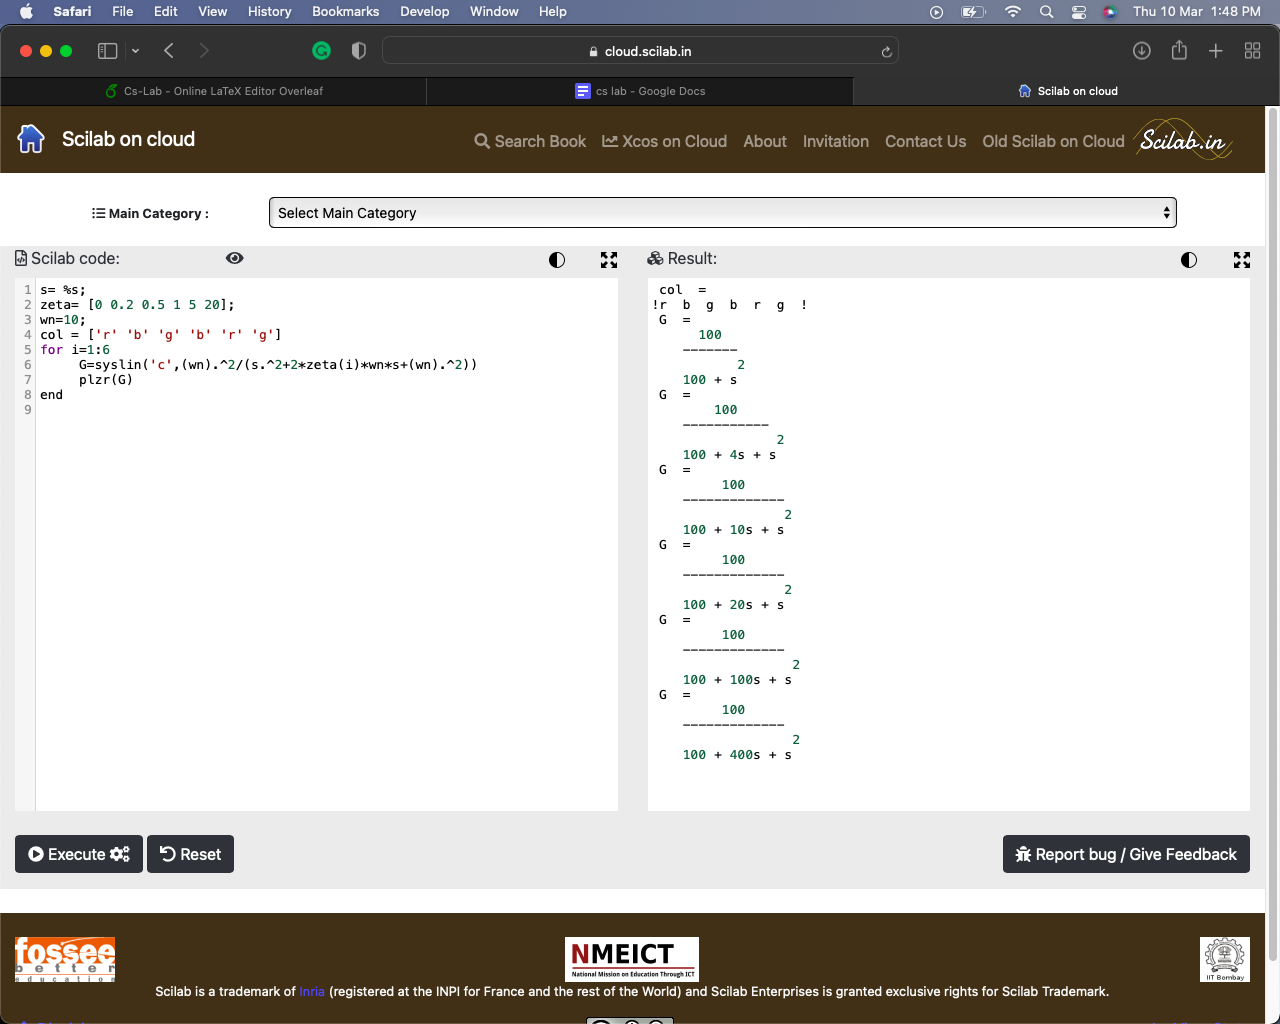
\includegraphics[width =10cm, height = 10cm]{images/exp132.png}
        \caption{Graph}
        \label{Result}
\end{figure}
\section*{\textcolor{black}{Conclusion}}
From the above analysis, it can be concluded that the closed-loop systems tend to be stable under certain conditions. the mere fact that all closed-loop poles lie in the left-half s plane does not guarantee satisfactory transient- response characteristics. If dominant complex-conjugate closed-loop poles lie close to the j axis, the transient response may exhibit excessive oscilla- tions or may be very slow. Therefore, to guarantee fast, yet well-damped, transient-response characteristics, it is necessary that the closed-loop poles of the system lie in a particular region in the complex plane.
 \pagebreak

\end{document}
